%
% TCC II - NO-FIS
% Categorização automática de itens de notas fiscais de consumidor
%
% Baseado no modelo LaTeX de monografia UNISINOS (TCC_V2.tex / exemplo.tex).
%
% Marcadores usados neste arquivo:
%   % TODO:     trecho que precisa ser revisado ou reescrito
%   % CONFERIR: informação que precisa ser verificada na fonte
%

%=======================================================================
% Declarações iniciais
%=======================================================================
\documentclass[english,brazilian]{UNISINOSmonografia}
\usepackage[utf8]{inputenc} % charset do texto (utf8, latin1, etc.)
\usepackage[T1]{fontenc} % encoding da fonte (afeta a sep. de sílabas)
\usepackage{graphicx} % comandos para gráficos e inclusão de figuras
\usepackage{bibentry} % para inserir refs. bib. no meio do texto
\usepackage{amsmath} % equações (silhueta, K-Means, HDBSCAN)
\usepackage{tabularx} % tabelas com largura do texto
\usepackage{hyperref}

\unisinosbst

%=======================================================================
% Dados gerais sobre o trabalho.
%=======================================================================
\autor{Simão}{Samuel}
\titulo{NO-FIS}
\subtitulo{Categorização automática de itens de notas fiscais de consumidor}
\orientador[Prof.]{Chagas Kurtz}{Guilherme}

\unidade{Unidade Acadêmica de Graduação ou Unidade Acadêmica de Educação Online}
\curso{Bacharelado em Sistemas de Informação}
\nivel{Graduação}
\natureza{Trabalho de Conclusão de Curso apresentado como requisito parcial para a obtenção do título de Bacharel em Sistemas de Informação, pelo Curso de Sistemas de Informação da Universidade do Vale do Rio dos Sinos --- UNISINOS}
\local{São Leopoldo}
\ano{2026}

% TODO: revisar palavras-chave (taxonomia e LLMs saíram do escopo; avaliar
% incluir HDBSCAN, embeddings ou NCM).
\palavrachave{brazilian}{Notas fiscais}
\palavrachave{brazilian}{Processamento de Linguagem Natural}
\palavrachave{brazilian}{Aprendizado de máquina não supervisionado}
\palavrachave{brazilian}{Clusterização}
\palavrachave{brazilian}{Taxonomia de produtos}

\palavrachave{english}{Electronic invoices}
\palavrachave{english}{Natural Language Processing}
\palavrachave{english}{Unsupervised machine learning}
\palavrachave{english}{Clustering}
\palavrachave{english}{Product taxonomy}


%=======================================================================
% Início do documento.
%=======================================================================
\begin{document}
\capa
\folhaderosto


%=======================================================================
% Resumo em Português.
%=======================================================================
% TODO: reescrever o resumo. O texto abaixo é o do TCC I e ainda descreve
% K-Means, LLMs e taxonomia como abordagem principal. O TCC II comparou
% TF-IDF, embeddings e representação híbrida com K-Means, DBSCAN e HDBSCAN.
\begin{abstract}
A descrição dos produtos presentes em notas fiscais eletrônicas de consumidor constitui uma fonte relevante para aplicações de análise de consumo, organização de despesas e estruturação de bases de dados. Entretanto, esse campo costuma ser registrado em formato livre pelos estabelecimentos comerciais, resultando em textos curtos, ruidosos, abreviados e pouco padronizados. Essa característica dificulta a identificação automática de produtos semelhantes e a associação desses itens a categorias interpretáveis. Diante desse problema, este trabalho propõe uma abordagem para apoiar a construção de uma taxonomia plana de categorias de produtos a partir de descrições extraídas de notas fiscais eletrônicas, utilizando técnicas de Processamento de Linguagem Natural, Aprendizado de Máquina não supervisionado e Modelos de Linguagem de Grande Escala. A metodologia prevê a coleta e estruturação de dados de itens fiscais, o pré-processamento das descrições textuais, a representação dos textos por meio de TF-IDF com \textit{n-grams} de palavras e caracteres e a aplicação do algoritmo K-Means para formação de agrupamentos de descrições semelhantes. Após a clusterização, serão selecionados exemplos representativos de cada agrupamento, os quais servirão de insumo para a sugestão de rótulos com apoio de Modelos de Linguagem de Grande Escala. Esses rótulos serão avaliados e ajustados por meio de validação humana, considerando critérios como coerência interna dos clusters, clareza dos nomes sugeridos e adequação das categorias à taxonomia proposta. A avaliação dos resultados combinará métricas internas de clusterização, como coeficiente de silhueta, índice Calinski-Harabasz e índice Davies-Bouldin, com análise qualitativa da interpretabilidade dos agrupamentos. Como resultado esperado, busca-se obter uma taxonomia inicial de categorias de produtos e um protótipo capaz de realizar a categorização inicial de novas descrições, contribuindo para a organização automática de itens de notas fiscais eletrônicas.
\end{abstract}


%=======================================================================
% Resumo em língua estrangeira.
%=======================================================================
% TODO: atualizar o abstract junto com o resumo.
\begin{otherlanguage}{english}
\begin{abstract}
Product descriptions found in electronic consumer invoices represent a relevant source of data for applications such as consumption analysis, expense organization and database structuring. However, this field is usually recorded in free-text format by commercial establishments, resulting in short, noisy, abbreviated and poorly standardized descriptions. This characteristic makes it difficult to automatically identify similar products and associate these items with interpretable categories. Given this problem, this work proposes an approach to support the construction of a flat taxonomy of product categories from descriptions extracted from electronic invoices, using Natural Language Processing techniques, unsupervised Machine Learning and Large Language Models. The proposed methodology includes the collection and structuring of invoice item data, textual preprocessing of product descriptions, text representation through TF-IDF with word and character \textit{n-grams}, and the application of the K-Means algorithm to form groups of similar descriptions. After clustering, representative examples from each group will be selected and used as input for label suggestions supported by Large Language Models. These labels will be evaluated and adjusted through human validation, considering criteria such as internal coherence of the clusters, clarity of the suggested names and suitability of the categories for the proposed taxonomy. The evaluation of the results will combine internal clustering metrics, such as the silhouette coefficient, the Calinski-Harabasz index and the Davies-Bouldin index, with a qualitative analysis of the interpretability of the groups. As an expected result, this work aims to obtain an initial taxonomy of product categories and a prototype capable of performing the initial categorization of new descriptions, contributing to the automatic organization of items from electronic invoices.
\end{abstract}
\end{otherlanguage}


%=======================================================================
% Listas
%=======================================================================
\listoffigures

\listoftables

%=======================================================================
% Sumário
%=======================================================================
\tableofcontents




%=======================================================================
% Introdução
%=======================================================================
% Mantida sem alterações em relação ao TCC I, exceto pela seção Objetivos.
% TODO (autor): ajustar introdução e justificativa ao escopo do TCC II
% (o último parágrafo ainda menciona LLMs e taxonomia).
\chapter{Introdução}

A digitalização dos documentos fiscais no Brasil possibilitou a geração, o armazenamento e a consulta eletrônica de informações relacionadas a operações comerciais. Segundo \cite{sefazrsnfe}, a Nota Fiscal Eletrônica (NF-e) foi criada com o objetivo de substituir documentos fiscais em papel por documentos digitais com validade jurídica, trazendo benefícios como redução de custos, simplificação de obrigações acessórias e maior agilidade no acesso às informações fiscais. De modo geral, os documentos fiscais eletrônicos registram dados como informações do estabelecimento emissor, valores da compra, tributos, forma de pagamento e relação dos produtos adquiridos.

As informações presentes nesses documentos representam uma fonte de dados com potencial para diferentes aplicações, como controle financeiro pessoal, análise de consumo, organização de despesas e estruturação de bases de dados a partir de documentos fiscais. Em especial, os itens das notas fiscais permitem identificar os produtos adquiridos por meio de suas descrições textuais. Contudo, embora esses documentos possuam diversos campos estruturados, a descrição dos produtos é registrada em formato livre, de acordo com os padrões adotados por cada estabelecimento comercial. Como destacado por \cite{santos2023classificacao}, essas descrições podem ser consideradas textos não estruturados, pois apresentam variações de escrita, abreviações e ausência de padronização.

Essa falta de padronização faz com que produtos semelhantes sejam descritos de formas distintas. Um mesmo produto pode aparecer com variações relacionadas à marca, quantidade, unidade de medida, abreviações, pontuação ou termos específicos utilizados pelo varejo. Por exemplo, descrições como ``REFRI COCA 2L'', ``COCA COLA PET 2LT'', ``COCA-COLA 2 LITROS'' e ``REFRIG COCA 2L'' podem se referir a produtos semelhantes, embora apresentem diferenças textuais relevantes. Essas variações dificultam o processamento automático e tornam mais complexa a identificação de padrões entre os itens.

Além disso, a descrição textual do produto não indica diretamente uma categoria de produto. Dessa forma, há uma dificuldade em utilizar essas informações em aplicações que dependem da organização dos itens em grupos interpretáveis, como alimentos, bebidas, higiene, limpeza, vestuário ou outras categorias de produtos. A ausência de categorias padronizadas impede que essas descrições sejam diretamente utilizadas em análises agregadas de consumo, organização de despesas ou estruturação de bases categorizadas. Como consequência, a organização desses dados tende a passar por processos manuais, regras específicas ou classificações construídas caso a caso, que podem ser difíceis de manter diante da grande variedade de descrições existentes.

Esse processo é desafiador porque as descrições dos produtos são curtas, ruidosas, pouco padronizadas e, na maioria dos casos, não possuem categorias previamente atribuídas. Assim, para categorizar ou organizar automaticamente esses itens em grupos compreensíveis, torna-se necessário investigar formas de descobrir padrões entre descrições semelhantes e transformá-los em categorias interpretáveis.

Nesse contexto, técnicas de Processamento de Linguagem Natural podem ser utilizadas para apoiar o tratamento dessas descrições. Por meio de etapas de pré-processamento textual e representação numérica, descrições de produtos podem ser convertidas em vetores capazes de representar padrões textuais relevantes. Essas representações tornam possível a aplicação de técnicas computacionais voltadas à análise de similaridade entre descrições, permitindo explorar relações que não são evidentes quando os textos são observados apenas em sua forma original.

A utilização de técnicas não supervisionadas torna-se adequada nesse cenário porque permite explorar padrões presentes nos dados sem depender de categorias previamente definidas. Em vez de partir de uma estrutura classificatória pronta, a análise dos agrupamentos pode revelar aproximações entre descrições de produtos e indicar possíveis formas de organização dos itens. Assim, a clusterização aparece como uma estratégia de apoio à investigação inicial das categorias, contribuindo para transformar um conjunto amplo de descrições livres em grupos mais interpretáveis.

Entretanto, a formação automática de agrupamentos não resolve integralmente o problema da categorização. Embora algoritmos de clusterização possam aproximar descrições textualmente semelhantes, os grupos resultantes ainda precisam ser interpretados para que façam sentido no domínio analisado. Essa etapa exige compreender o conteúdo predominante de cada agrupamento e relacioná-lo a categorias úteis para a organização dos produtos. Nesse ponto, os Modelos de Linguagem de Grande Escala podem atuar como apoio à interpretação dos grupos, auxiliando na sugestão de nomes mais compreensíveis e próximos da linguagem utilizada por humanos.

Dessa forma, a taxonomia de categorias de produtos é compreendida, neste trabalho, como uma estrutura de organização capaz de tornar as descrições dos itens fiscais mais interpretáveis e úteis para análises posteriores. Considerando que os documentos fiscais eletrônicos não fornecem, de forma padronizada, uma categoria associada a cada produto descrito, torna-se necessário investigar alternativas que apoiem a organização dessas descrições em grupos compreensíveis.

Diante disso, este trabalho é motivado pela necessidade de investigar uma abordagem capaz de apoiar a construção de uma taxonomia plana de categorias de produtos a partir de descrições curtas, ruidosas e não padronizadas extraídas de documentos fiscais eletrônicos. A pesquisa busca responder à seguinte questão: como técnicas de Processamento de Linguagem Natural, Aprendizado de Máquina não supervisionado e Modelos de Linguagem de Grande Escala podem apoiar a construção de uma taxonomia plana de categorias de produtos a partir de descrições curtas e não padronizadas extraídas de documentos fiscais eletrônicos?



\section{Objetivos}

\subsection{Objetivo geral}

Desenvolver e avaliar uma abordagem para a categorização automática de descrições de produtos presentes em notas fiscais eletrônicas, utilizando técnicas de Processamento de Linguagem Natural e Aprendizado de Máquina não supervisionado para identificar agrupamentos de produtos semelhantes e associar novas descrições a categorias de produtos.

\subsection{Objetivos específicos}

\begin{alineas}
    \item coletar, explorar e preparar descrições de produtos extraídas de notas fiscais eletrônicas, com foco em produtos comercializados em supermercados;
    \item investigar e comparar diferentes técnicas de representação textual, como TF-IDF e \textit{embeddings} semânticos;
    \item avaliar algoritmos de clusterização para identificar agrupamentos de descrições de produtos semelhantes;
    \item analisar e interpretar os agrupamentos identificados, estabelecendo sua associação a categorias de produtos;
    \item desenvolver um protótipo capaz de categorizar novas descrições de produtos a partir dos agrupamentos identificados, apresentando a categoria atribuída e exemplos representativos;
    \item avaliar a qualidade dos agrupamentos e da categorização de novas descrições, considerando métricas quantitativas e a coerência semântica dos resultados.
\end{alineas}




%=======================================================================
% Referencial Teórico
%=======================================================================
\chapter{Referencial Teórico}

Este capítulo apresenta os conceitos que fundamentam a análise de descrições de produtos em documentos fiscais. São abordados os documentos fiscais eletrônicos e a Nomenclatura Comum do Mercosul (NCM), o Processamento de Linguagem Natural e as representações textuais TF-IDF e por \textit{embeddings}. Em seguida, são discutidos o aprendizado não supervisionado, os algoritmos de clusterização utilizados e as métricas adotadas para avaliar seus resultados. Por fim, apresenta-se o t-SNE como recurso de visualização dos agrupamentos.

\section{Notas fiscais de consumidor eletrônicas no Brasil}

A Nota Fiscal Eletrônica (NF-e) e a Nota Fiscal de Consumidor Eletrônica (NFC-e) são documentos fiscais digitais utilizados para registrar operações com mercadorias. A NF-e corresponde ao modelo 55; a NFC-e, ao modelo 65, voltado às operações de venda ao consumidor final. Embora tenham finalidades distintas, ambos organizam as informações dos itens em campos como código, descrição, quantidade, unidade de medida e valor, como ilustra a Figura~\ref{fig:DANFE}. Essa estrutura permite identificar os produtos registrados em uma operação, mas não torna uniforme a forma como eles são descritos \cite{sefazsp-nfe,encat2025manual}.

% Imagem extraída do TCC II.docx.
\begin{figure}[htbp]
    \caption{Exemplo de DANFE NFC-e}
    \label{fig:DANFE}
    \centering
    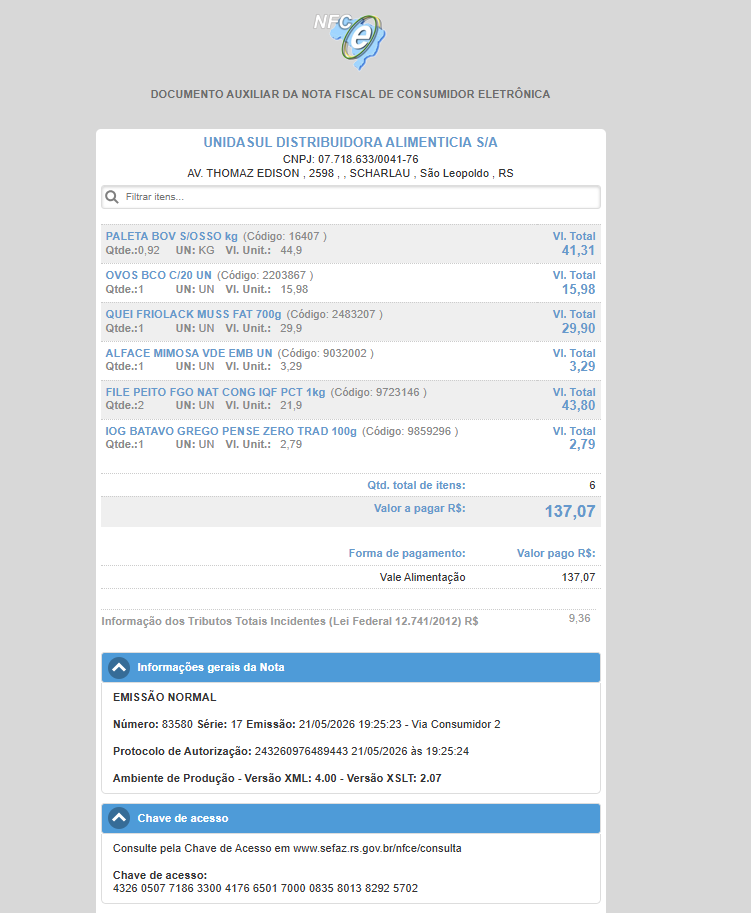
\includegraphics[width=0.6\linewidth]{images/danfe-nfce.png}
    \fonte{O Autor}
\end{figure}

O campo de descrição reúne informações relevantes em poucas palavras, frequentemente com abreviações, marcas, medidas e características de apresentação. Uma mesma mercadoria pode aparecer sob nomes diferentes, enquanto descrições parecidas podem corresponder a produtos distintos. Assim, a regularidade dos campos do documento fiscal convive com a variação da linguagem utilizada para preencher cada descrição. Essa diferença explica por que a análise automática dos itens depende de técnicas capazes de comparar textos curtos e pouco padronizados.

\section{Nomenclatura Comum do Mercosul (NCM)}

A Nomenclatura Comum do Mercosul (NCM) é um sistema utilizado para a classificação de mercadorias nos países integrantes do Mercosul. Segundo a Receita Federal do Brasil, uma nomenclatura consiste em um sistema ordenado que, por meio de regras e procedimentos próprios, permite determinar um código numérico para representar determinada mercadoria. A NCM é adotada por Brasil, Argentina, Paraguai e Uruguai desde 1995 e tem como base o Sistema Harmonizado de Designação e de Codificação de Mercadorias (SH), mantido pela Organização Mundial das Alfândegas (OMA) \cite{brasil2024ncm}.

Os códigos da NCM são formados por oito dígitos e apresentam uma estrutura hierárquica. Os seis primeiros dígitos seguem o Sistema Harmonizado, enquanto os dois últimos correspondem a desdobramentos definidos no âmbito do Mercosul. A organização compreende níveis de posição, com quatro dígitos, subposição, com cinco ou seis dígitos, item, com sete dígitos, e subitem, correspondente ao código completo de oito dígitos. Além disso, a nomenclatura está distribuída em seções e capítulos que organizam as mercadorias segundo suas características e grau de elaboração \cite{brasil2024ncm}.

Essa estrutura permite observar diferentes níveis de generalidade na classificação. Dessa forma, códigos que compartilham os mesmos dígitos iniciais tendem a pertencer a agrupamentos mais amplos da nomenclatura, enquanto o avanço para os níveis de item e subitem aumenta a especificidade da identificação da mercadoria. A classificação fiscal, entretanto, não depende apenas da comparação textual entre nomes de produtos, pois deve considerar as regras da NCM, as características da mercadoria, sua composição, finalidade e as notas legais aplicáveis à classificação \cite{brasil2024ncm}.

A consulta à nomenclatura pode ser realizada por meio do Sistema Classif, disponibilizado no Portal Único de Comércio Exterior. O sistema possibilita pesquisar mercadorias pelo código ou por palavras, além de navegar pela estrutura hierárquica da NCM. A plataforma também disponibiliza a tabela vigente, suas notas legais e explicativas e permite obter os dados da nomenclatura em formatos estruturados, como JSON e XLSX \cite{brasil2025classif}.

Em bases de notas fiscais, o NCM é uma informação estruturada que pode auxiliar na identificação e seleção inicial de mercadorias. Sua finalidade é a classificação fiscal, com usos como determinação de tributos, tratamentos administrativos e produção de estatísticas. No projeto, o NCM é tratado como informação auxiliar sobre os itens, e não como rótulo de similaridade textual: os agrupamentos são formados a partir das descrições dos produtos.

\section{Processamento de Linguagem Natural}

O Processamento de Linguagem Natural (PLN) é uma área da ciência da computação voltada ao tratamento computacional da linguagem humana. Como os computadores não operam diretamente sobre o significado das palavras da mesma forma que os seres humanos, os textos precisam ser processados e representados de modo que seus padrões possam ser analisados por algoritmos. Segundo a \cite{ibm2024pln}, o PLN é um subcampo da ciência da computação que utiliza técnicas de aprendizado de máquina para permitir que computadores interpretem e se comuniquem por meio da linguagem humana.

No contexto deste trabalho, o PLN é relevante porque as descrições dos itens presentes em notas fiscais são formadas por textos em linguagem natural, frequentemente curtos, abreviados e pouco padronizados. Para que essas descrições possam ser utilizadas na organização automática e na categorização inicial de produtos, é necessário submetê-las a etapas de tratamento e transformação que permitam aos modelos identificar padrões textuais associados a grupos de itens semelhantes.

Dessa forma, o PLN permite transformar descrições livres de produtos em representações processáveis computacionalmente. Essas representações são utilizadas pelos algoritmos não supervisionados para analisar semelhanças entre descrições e formar agrupamentos.

\section{Representação de textos para modelos de aprendizado de máquina}

Para que textos possam ser utilizados como entrada em modelos de aprendizado de máquina, é necessário transformá-los em uma representação estruturada e processável computacionalmente. Isso ocorre porque algoritmos de aprendizado de máquina não operam diretamente sobre o texto em sua forma bruta, mas sobre atributos numéricos extraídos desses textos. Segundo \cite{manning2008informationretrieval}, o processamento textual envolve etapas como a definição da unidade documental, a tokenização, o pré-processamento linguístico dos tokens e a construção de um vocabulário de termos.

No contexto deste trabalho, cada descrição de produto extraída da nota fiscal pode ser tratada como um documento textual. Assim, uma descrição como ``COCA COLA PET 2L'' é considerada uma unidade de análise que precisa ser convertida em uma representação numérica. A tokenização consiste em dividir essa sequência de caracteres em unidades menores, chamadas tokens, que podem corresponder a palavras, partes de palavras, números ou sequências de caracteres, dependendo da estratégia adotada. Após essa etapa, os tokens podem ser normalizados e utilizados para formar um vocabulário, isto é, o conjunto de termos considerados relevantes no corpus analisado.

Existem diferentes formas de representar textos numericamente, variando desde modelos mais simples, baseados na ocorrência de palavras, até estratégias que consideram combinações de termos ou sequências de caracteres. Entre essas formas, destacam-se a representação por \textit{n-grams} e a ponderação TF-IDF (\textit{Term Frequency-Inverse Document Frequency}). Essas técnicas são relevantes para este trabalho porque permitem transformar descrições curtas e não padronizadas de produtos em vetores numéricos que poderão ser utilizados posteriormente pelos algoritmos de clusterização.

\subsection{N-gramas de palavras e caracteres}

Um n-grama é uma sequência contígua de $n$ unidades de texto. Quando as unidades são palavras, a sequência pode registrar expressões como ``leite integral'', distinguindo-as de palavras consideradas isoladamente. Quando são caracteres, n-gramas permitem representar partes de uma palavra e reconhecer alguma sobreposição entre formas abreviadas, variantes de escrita e pequenas diferenças de grafia.

Essas duas formas de segmentação capturam informações complementares. Os n-gramas de palavras preservam associações entre termos vizinhos; os de caracteres reduzem a dependência de palavras exatamente iguais. Em contrapartida, sequências de caracteres compartilhadas também podem aproximar termos de significado diferente, e o aumento do número de sequências possíveis amplia o espaço de atributos. A semelhança observada continua, portanto, ligada à forma escrita dos textos \cite{manning2008informationretrieval}.

\subsection{Ponderação TF-IDF}

Após a definição dos termos ou \textit{n-grams}, é necessário atribuir valores numéricos a eles. Uma alternativa simples seria utilizar apenas a frequência absoluta dos termos em cada documento. No entanto, essa estratégia pode atribuir muita importância a termos que aparecem com frequência em vários documentos, mas que possuem baixo poder discriminativo. Para reduzir esse problema, pode-se utilizar a ponderação TF-IDF, do inglês \textit{Term Frequency-Inverse Document Frequency}. Segundo \cite{ramos2003tfidf}, a combinação entre frequência do termo e frequência inversa nos documentos permite estimar a importância de um termo para a representação de um documento dentro de uma coleção.

O TF-IDF combina duas informações principais. A primeira é a frequência do termo no documento, chamada de TF (\textit{Term Frequency}), que indica o quanto determinado termo aparece em uma descrição. A segunda é a frequência inversa nos documentos, chamada de IDF (\textit{Inverse Document Frequency}), que reduz o peso de termos muito frequentes no conjunto total de documentos e aumenta o peso de termos mais específicos. Assim, o peso TF-IDF de um termo tende a ser maior quando ele aparece com frequência em um documento específico, mas não aparece em muitos documentos da coleção.

Assim, um termo que aparece muitas vezes em uma descrição, mas também aparece em grande parte da base, tende a receber um peso menor. Por outro lado, um termo que aparece em menos documentos, mas é relevante para identificar um grupo específico de produtos, tende a receber um peso maior.

De forma geral, a ponderação TF-IDF valoriza termos frequentes em um documento que não aparecem em todos os documentos da coleção. Nas descrições de produtos, termos recorrentes podem contribuir pouco para distinguir grupos, enquanto termos mais específicos, marcas, unidades de medida e combinações características podem ajudar os algoritmos a identificar padrões textuais.

Dessa forma, a combinação entre \textit{n-grams} e TF-IDF permite transformar descrições textuais curtas em vetores numéricos que preservam parte das características relevantes dos produtos. Esses vetores podem então ser utilizados por algoritmos de aprendizado de máquina, especialmente em tarefas de agrupamento, nas quais o objetivo é identificar descrições textualmente semelhantes e organizá-las em grupos interpretáveis.

\subsection{Embeddings de sentenças e modelo multilíngue}

\textit{Embeddings} de sentenças representam textos por vetores densos, de modo que relações entre os vetores possam ser utilizadas para comparar as descrições. Em modelos voltados à similaridade de sentenças, o treinamento busca aproximar textos semanticamente relacionados, permitindo investigar semelhanças que não dependem apenas da coincidência literal das palavras \cite{reimers2019sentencebert}.

O modelo \texttt{sentence-transformers/paraphrase-multilingual-mpnet-base-v2} produz vetores de 768 dimensões e oferece suporte multilíngue. Embora seu identificador contenha ``mpnet'', a arquitetura publicada dessa versão utiliza um codificador XLM-RoBERTa, seguido de agregação pela média das representações dos tokens \cite{sentencetransformers-mpnet,conneau2020xlmr}. Neste trabalho, MPNet é utilizado como denominação abreviada desse modelo específico, sem atribuir a ele a arquitetura do MPNet original.

A proximidade entre \textit{embeddings} oferece uma forma de investigar relações entre descrições com vocabulários diferentes. Entretanto, a semelhança vetorial precisa ser interpretada no domínio dos produtos. Informações de marca, medida ou apresentação podem ser relevantes para distinguir mercadorias, e a utilidade da representação depende da análise dos agrupamentos produzidos.

\section{Aprendizado não supervisionado e clusterização}

Métodos de aprendizado de máquina podem ser classificados de acordo com a forma como os dados são utilizados durante o processo de aprendizagem. No aprendizado supervisionado, os exemplos utilizados no treinamento possuem rótulos ou valores-alvo previamente conhecidos. Nesse caso, o objetivo do algoritmo é aprender uma relação entre as entradas e as saídas esperadas, permitindo classificar ou prever novos exemplos. No aprendizado não supervisionado, por outro lado, os dados não possuem rótulos previamente atribuídos, e o objetivo é identificar estruturas, padrões ou relações existentes na própria distribuição dos dados.

No contexto deste trabalho, o aprendizado não supervisionado é especialmente relevante porque as descrições dos produtos extraídas das notas fiscais não possuem, inicialmente, categorias previamente definidas. Dessa forma, não há uma base rotulada que permita treinar diretamente um classificador supervisionado. Em vez disso, busca-se explorar as descrições disponíveis para identificar grupos de itens semelhantes, que possam servir como apoio à descoberta de categorias e à construção de uma taxonomia de produtos.

Uma das principais técnicas associadas ao aprendizado não supervisionado é a clusterização. Segundo \cite{tan2005introduction}, a análise de clusters tem como objetivo dividir os dados em grupos, chamados \textit{clusters}, que sejam significativos, úteis ou ambos. Quando o objetivo é identificar grupos significativos, espera-se que os clusters capturem estruturas naturais presentes nos dados. Em outras situações, a clusterização pode ser utilizada como ponto de partida para outras tarefas, como sumarização dos dados, organização de documentos ou apoio à análise exploratória.

De modo geral, uma boa clusterização busca formar grupos em que os objetos pertencentes ao mesmo cluster sejam semelhantes ou relacionados entre si, enquanto objetos pertencentes a clusters diferentes sejam menos semelhantes ou não relacionados. Assim, quanto maior a homogeneidade interna dos grupos e maior a separação entre grupos distintos, mais clara tende a ser a estrutura de clusterização obtida.

No entanto, a definição de um cluster nem sempre é precisa. Um mesmo conjunto de dados pode ser dividido de diferentes formas, dependendo do algoritmo utilizado, da medida de similaridade adotada, dos parâmetros escolhidos e do objetivo da análise. Por esse motivo, a clusterização deve ser entendida como uma técnica exploratória, cuja interpretação depende tanto dos resultados computacionais quanto da análise do contexto do problema.

% TODO: parágrafo herdado do TCC I; atualizar para incluir embeddings e
% usar o tempo verbal do trabalho realizado.
No caso deste trabalho, cada descrição de produto será representada numericamente por meio de técnicas de Processamento de Linguagem Natural, como TF-IDF e \textit{n-grams}. A partir dessas representações vetoriais, algoritmos de clusterização poderão agrupar descrições textualmente semelhantes. Por exemplo, descrições como ``coca cola pet 2l'', ``refrigerante cola 2lt'' e ``guarana lata 350ml'' podem ser aproximadas caso compartilhem padrões textuais relevantes. Por outro lado, descrições como ``sabao po 1kg'', ``arroz branco 5kg'' e ``creme dental 90g'' tendem a pertencer a agrupamentos diferentes, caso a representação textual e o algoritmo utilizado consigam capturar tais diferenças.

\section{Algoritmos de clusterização}

A clusterização busca identificar conjuntos de observações semelhantes sem utilizar rótulos prévios. O significado de ``semelhança'' depende da representação dos dados, da medida de distância e da definição de cluster adotada pelo algoritmo. Entre as abordagens mais conhecidas estão os métodos baseados em centroides, representados aqui pelo K-Means, e os métodos baseados em densidade, como DBSCAN e HDBSCAN. Essa distinção é relevante para descrições textuais: um grupo de vetores próximos de um centro pode ter estrutura diferente de uma região formada por descrições localmente próximas entre si \cite{tan2005introduction}.

\subsection{K-Means}

O K-Means é um algoritmo particional que divide os dados em $k$ grupos não sobrepostos. Cada grupo $C_j$ é representado por um centroide $\mu_j$, definido pela média dos vetores que lhe são atribuídos. O objetivo do algoritmo é minimizar a soma das distâncias euclidianas quadráticas entre cada vetor $x_i$ e o centroide de seu grupo:
\begin{equation}
J=\sum_{j=1}^{k}\sum_{x_i\in C_j}\lVert x_i-\mu_j\rVert_2^2.
\label{eq:kmeans}
\end{equation}

Para reduzir essa soma, o algoritmo alterna duas etapas: atribui cada vetor ao centroide mais próximo e recalcula os centroides a partir dos grupos formados. A repetição termina quando as atribuições se estabilizam ou quando é atingido um critério de parada. Como o resultado pode depender dos centroides iniciais, diferentes inicializações podem produzir partições distintas e levar a mínimos locais da função objetivo \cite{tan2005introduction}.

A quantidade de grupos precisa ser definida antes do ajuste. Um valor pequeno de $k$ pode reunir padrões diferentes em um mesmo cluster; um valor grande pode dividir padrões próximos em grupos separados. O K-Means também atribui todas as observações a algum centroide, inclusive aquelas afastadas dos demais pontos. Por utilizar médias como representantes, tende a descrever melhor grupos compactos em torno de centros. No agrupamento de textos, essas propriedades devem ser interpretadas no espaço vetorial produzido pela representação textual, e não diretamente a partir das palavras originais.

\subsection{DBSCAN}

O DBSCAN define clusters a partir de regiões de alta densidade separadas por regiões menos densas \cite{ester1996dbscan}. Uma observação é considerada central quando sua vizinhança de raio $\varepsilon$ contém uma quantidade mínima de pontos, definida por \textit{MinPts}. A partir de um ponto central, o algoritmo expande o grupo para outros pontos centrais alcançáveis por sequências de vizinhanças. Pontos próximos de um grupo, mas sem vizinhos suficientes para expandi-lo, são pontos de borda; os que não são incorporados a nenhum grupo recebem a identificação de ruído.

Essa definição permite que um cluster tenha formato irregular e dispensa a escolha prévia de sua quantidade, como ilustra a Figura~\ref{fig:dbscan}. A identificação de ruído também expressa uma diferença conceitual em relação ao K-Means: uma observação isolada pode permanecer sem grupo quando não há densidade suficiente à sua volta. O resultado depende, contudo, da escala de vizinhança estabelecida por $\varepsilon$ e da densidade mínima exigida por \textit{MinPts}. Um raio muito pequeno pode fragmentar grupos e aumentar o ruído; um raio muito grande pode unir regiões distintas.

\begin{figure}[htbp]
    \caption{Agrupamentos de formatos irregulares identificados pelo DBSCAN}
    \label{fig:dbscan}
    \centering
    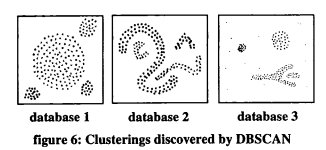
\includegraphics[width=0.6\linewidth]{images/dbscan-ester1996.png}
    \fonte{\citetexto{ester1996dbscan}}
\end{figure}

Como o DBSCAN usa um mesmo limiar de vizinhança para todo o conjunto, grupos com densidades muito diferentes podem ser difíceis de recuperar simultaneamente. A dificuldade também cresce quando as distâncias entre observações se tornam pouco discriminativas, situação possível em espaços vetoriais de alta dimensionalidade. Por isso, a escolha da representação e da distância participa da própria definição das regiões consideradas densas.

\subsection{HDBSCAN}

O HDBSCAN desenvolve a ideia de agrupamento por densidade ao examinar a estrutura dos dados em múltiplas escalas, em vez de selecionar um único valor de $\varepsilon$ \cite{campello2013hdbscan}. Para cada ponto, calcula-se a distância necessária para alcançar o número mínimo de vizinhos exigido, chamada distância de núcleo. A distância de alcançabilidade mútua entre dois pontos $x$ e $y$ é o maior valor entre a distância original e suas distâncias de núcleo:
\begin{equation}
d_{\mathrm{mr}}(x,y)=\max\{d_{\mathrm{core}}(x),\, d_{\mathrm{core}}(y),\, d(x,y)\}.
\label{eq:hdbscan}
\end{equation}
Esse ajuste reduz a influência de conexões que passam por regiões pouco densas.

A partir dessas proximidades, o algoritmo constrói uma hierarquia: conforme o nível de densidade varia, grupos podem surgir, dividir-se ou desaparecer. A hierarquia é condensada para descartar grupos menores que um tamanho mínimo, e uma medida de estabilidade permite selecionar clusters que persistem ao longo de diferentes níveis de densidade. Desse modo, a solução final pode reunir grupos identificados em escalas distintas, sem definir antecipadamente sua quantidade \cite{campello2013hdbscan}.

O tamanho mínimo do cluster e o número de observações considerado na estimativa da densidade local influenciam a estrutura obtida e a identificação de ruído. Embora a análise hierárquica permita examinar densidades diferentes, ela não elimina a dependência da representação vetorial nem garante que todo grupo encontrado seja semanticamente homogêneo. Assim como no DBSCAN, uma parte das observações pode permanecer sem cluster.

\section{Avaliação dos agrupamentos}

Na ausência de rótulos de referência, a avaliação interna examina relações entre os vetores e as atribuições produzidas pelo algoritmo. O coeficiente de silhueta \cite{rousseeuw1987silhouettes} considera, para cada observação $i$, a distância média $a_i$ aos elementos de seu próprio cluster e a menor distância média $b_i$ aos elementos de outro cluster. A medida subtrai a primeira distância da segunda e divide o resultado pela maior delas:
\begin{equation}
s_i=\frac{b_i-a_i}{\max\{a_i,\, b_i\}}.
\label{eq:silhueta}
\end{equation}
Seu valor varia de menos um a um; valores positivos elevados indicam maior separação segundo a distância adotada, enquanto valores próximos de zero indicam menor distinção entre grupos \cite{sklearn-silhouette}.

Nos métodos que identificam ruído, a silhueta calculada apenas entre observações agrupadas descreve a parcela que recebeu um cluster. Por isso, sua interpretação deve acompanhar a cobertura, definida como a fração de observações incluídas nos grupos, e a proporção complementar de ruído. Uma configuração pode formar poucos grupos bem separados e deixar grande parte dos dados sem atribuição.

A quantidade de clusters também deve ser relacionada ao nível de organização pretendido. Entretanto, a definição de uma faixa aceitável depende do problema e do objetivo da análise. Um limite adotado para selecionar configurações é um critério operacional da pesquisa, e não uma garantia de que os grupos correspondam a categorias comerciais adequadas.

As métricas internas descrevem a geometria da representação. A verificação da coerência semântica requer examinar os produtos reunidos, os casos ambíguos e as diferenças entre grupos. Também é necessário distinguir um identificador de cluster de um nome de categoria: a associação entre ambos depende de interpretação e validação.

\subsection{Visualização dos clusters com t-SNE}

O t-SNE é uma técnica de visualização que representa observações de alta dimensionalidade em duas ou três dimensões, buscando preservar principalmente suas relações locais de vizinhança \cite{vandermaaten2008tsne}. Ao colorir os pontos pelos rótulos de um algoritmo, a projeção permite inspecionar as atribuições previamente obtidas.

A técnica não define os clusters e não deve ser utilizada como comprovação isolada de sua qualidade. Distâncias entre regiões afastadas, áreas ocupadas e espaços vazios na projeção não reproduzem necessariamente a estrutura global do espaço original. Sua utilização deve complementar a leitura das métricas e das descrições que compõem cada grupo.




%=======================================================================
% Trabalhos Relacionados
%=======================================================================
\chapter{Trabalhos Relacionados}

Os trabalhos relacionados a esta pesquisa envolvem abordagens de Processamento de Linguagem Natural, Aprendizado de Máquina não supervisionado, categorização de descrições fiscais e uso de Modelos de Linguagem de Grande Escala para apoiar a interpretação de agrupamentos textuais. Embora os estudos analisados tratem de problemas próximos, como classificação de textos, extração de informações em notas fiscais e rotulação automática de clusters, esta pesquisa se diferencia por investigar uma abordagem exploratória para apoiar a construção de uma taxonomia plana de categorias de produtos a partir de descrições curtas e não padronizadas de itens fiscais.

\cite{hajyahia2019unsupervised} apresentam uma abordagem de classificação não supervisionada de textos baseada no uso de conhecimento de especialistas e \textit{word embeddings}. O estudo parte de um cenário em que documentos bancários relacionados a incidentes de risco operacional precisavam ser organizados em uma nova taxonomia, sem que houvesse uma base previamente rotulada. Para isso, os autores modelam a tarefa como um problema de similaridade textual entre documentos e categorias previamente definidas, enriquecendo as categorias com palavras indicadas por especialistas, sinônimos e termos semanticamente próximos. Esse trabalho se relaciona com a presente pesquisa por abordar um contexto em que há textos não rotulados e necessidade de organização em categorias. No entanto, diferencia-se por partir de uma taxonomia previamente conhecida, enquanto a presente pesquisa busca apoiar a própria construção da taxonomia a partir dos agrupamentos encontrados nos dados.

No contexto de notas fiscais, \cite{martins2025extracao}, no trabalho ``Extração de Informação de Notas Fiscais apoiada em Conhecimento'', investiga o uso de técnicas de PLN, bases de conhecimento e Grandes Modelos de Linguagem para associar descrições presentes em notas fiscais a registros oficiais de medicamentos da Anvisa e da CMED. O estudo demonstra que descrições fiscais, embora sejam textos curtos, não estruturados e frequentemente inconsistentes, podem ser interpretadas com apoio de técnicas como reconhecimento e ligação de entidades, expressões regulares, filtragem de candidatos e LLMs. Uma contribuição relevante desse trabalho para a presente pesquisa é a constatação de que o uso isolado de Modelos de Linguagem de Grande Escala pode não ser suficiente para resolver todos os casos, reforçando a importância de combinar diferentes técnicas computacionais com etapas de validação e interpretação humana.

\cite{santos2023classificacao} propõe a classificação de produtos em Notas Fiscais Eletrônicas a partir de descrições textuais não estruturadas. O trabalho utiliza uma base de NF-e disponibilizada pelo Ministério Público do Estado da Paraíba e realiza a rotulação manual de uma amostra dos dados quanto à unidade de medida dos produtos. Em seguida, são comparadas duas abordagens: TF-IDF com SVM linear e o modelo \textit{tweet2vec}, baseado em redes neurais recorrentes em nível de caracteres. Os resultados indicam melhor desempenho da abordagem TF-IDF com SVM, evidenciando que métodos tradicionais de representação textual ainda podem ser eficazes em textos curtos e ruidosos. Esse estudo se aproxima da presente pesquisa por utilizar descrições de produtos em notas fiscais e por lidar com textos não padronizados. Contudo, diferencia-se por adotar uma abordagem supervisionada, dependente de rótulos manuais, enquanto esta pesquisa trabalha com um cenário exploratório, sem categorias previamente atribuídas aos itens.

A etapa de nomenclatura dos agrupamentos também se relaciona com o trabalho de \cite{murray2025using}, que discute o uso de modelos de linguagem para gerar rótulos descritivos para clusters de documentos. Os autores destacam que métodos tradicionais baseados apenas em termos distintivos podem gerar rótulos curtos ou pouco interpretáveis, enquanto modelos de linguagem podem produzir nomes mais próximos daqueles atribuídos por avaliadores humanos. Esse trabalho se aproxima diretamente da presente pesquisa no uso de LLMs como apoio à interpretação de clusters. Entretanto, enquanto \cite{murray2025using} trata da rotulação de clusters de documentos científicos, esta pesquisa aplica a ideia ao domínio de descrições curtas de produtos extraídos de notas fiscais eletrônicas, que apresentam características próprias, como abreviações, marcas, unidades de medida, números e variações de escrita.

De modo geral, os estudos analisados demonstram diferentes estratégias para lidar com textos curtos, não estruturados ou sem rotulação prévia. \cite{hajyahia2019unsupervised} exploram a classificação não supervisionada a partir de similaridade semântica com categorias previamente definidas; \cite{martins2025extracao} investigam a extração e ligação de informações em notas fiscais com apoio de conhecimento externo e LLMs; \cite{santos2023classificacao} avalia métodos supervisionados para classificação de descrições fiscais; e \cite{murray2025using} aborda o uso de modelos de linguagem na geração de rótulos para clusters textuais.

% TODO: parágrafo herdado do TCC I. Cita K-Means, LLMs e taxonomia; o TCC II
% comparou TF-IDF, embeddings e híbrido com K-Means, DBSCAN e HDBSCAN, e
% deixou a nomeação por LLM fora do escopo.
A presente pesquisa se diferencia desses trabalhos ao propor uma abordagem voltada à construção exploratória de uma taxonomia plana de categorias de produtos, partindo de descrições fiscais sem rótulos prévios. Para isso, combina técnicas de pré-processamento textual, representações TF-IDF com \textit{n-grams} de palavras e caracteres, clusterização com K-Means, seleção de exemplos representativos, apoio de LLMs para nomeação dos agrupamentos e validação humana dos rótulos propostos. Dessa forma, o foco não está apenas em classificar itens em categorias já existentes, mas em apoiar a descoberta, interpretação e organização inicial das categorias a partir dos próprios dados.




%=======================================================================
% Metodologia
%=======================================================================
\chapter{Metodologia}
\label{cap:metodologia}

Este capítulo apresenta os procedimentos utilizados para preparar as descrições de produtos e investigar a formação de agrupamentos por aprendizado de máquina não supervisionado. A pesquisa é de natureza aplicada, pois aborda um problema de organização e categorização de itens presentes em notas fiscais eletrônicas. Quanto aos procedimentos, possui caráter experimental, com a comparação de representações textuais e de configurações dos algoritmos K-Means, DBSCAN e HDBSCAN.

A implementação foi realizada em notebooks Python, organizados em etapas de coleta, exploração, seleção dos dados, pré-processamento, representação vetorial, agrupamento e análise. Inicialmente, foram examinadas representações TF-IDF e \textit{embeddings} semânticos com K-Means. Em seguida, foram explorados métodos baseados em densidade e projeções t-SNE para apoiar a inspeção dos dados. Também foi avaliada uma representação híbrida, combinando características das duas formas de representação.

\section{Base de dados}
\label{sec:base-dados}

A pesquisa utilizou os registros de notas fiscais disponibilizados pela Controladoria-Geral da União no Portal da Transparência do Governo Federal \cite{brasil2026notasfiscais}. A fonte reúne documentos relativos a aquisições de produtos e serviços pela Administração Pública Federal \cite{brasil2026entendanotas}. Foram considerados os arquivos dos doze meses de 2025. Os pacotes ZIP foram extraídos, e os arquivos CSV referentes aos itens foram convertidos para Parquet, formato utilizado nas etapas seguintes.

A unidade inicial de análise foi a linha correspondente a um item da nota fiscal. O campo textual utilizado foi ``DESCRIÇÃO DO PRODUTO/SERVIÇO''. Nos arquivos intermediários de 2025, foram contabilizados 7.639.476 registros, dos quais 5.979.164 continham descrição não vazia. Como a fonte inclui produtos de diferentes finalidades, foi necessário construir um recorte que aproximasse os tipos de mercadorias analisadas do domínio de produtos comercializados em supermercados.

O recorte foi definido por códigos da Nomenclatura Comum do Mercosul (NCM). Uma análise exploratória identificou 397 emissores candidatos por padrões textuais associados a supermercados e redes varejistas. Entre esses emissores, os dez com mais linhas de itens foram utilizados como referência para examinar os códigos presentes nas compras. Foram observados 453 NCMs distintos, dos quais foram mantidos aqueles com pelo menos cinco ocorrências. A lista resultante reuniu 241 códigos completos de oito dígitos.

A Tabela~\ref{tab:ncm} apresenta os quinze códigos mais frequentes nessa etapa de seleção. Suas contagens correspondem aos itens dos dez emissores de referência, e não à base anual completa.

\begin{table}[htbp]
    \caption{NCMs mais frequentes entre os emissores de referência}
    \label{tab:ncm}
    \centering
    \small
    \begin{tabularx}{\textwidth}{lXr}
        \hline
        \textbf{NCM} & \textbf{Descrição do tipo de produto} & \textbf{Linhas}\\
        \hline
        19059090 & Outros produtos de padaria, pastelaria e indústria de biscoitos & 889\\
        16010000 & Enchidos e produtos semelhantes de carne, miudezas ou sangue e preparações à base desses produtos & 840\\
        19053100 & Bolachas e biscoitos adicionados de edulcorante & 653\\
        22021000 & Águas adicionadas de açúcar, outros edulcorantes ou aromatizantes & 518\\
        17019900 & Outros açúcares de cana, beterraba ou sacarose & 345\\
        11010010 & Farinha de trigo & 344\\
        21069010 & Outras preparações para elaboração de bebidas & 337\\
        19052090 & Outros pães de especiarias & 319\\
        21039021 & Condimentos e temperos compostos em embalagens de até 1 kg & 259\\
        22029900 & Outras bebidas não alcoólicas, exceto água, cerveja sem álcool e itens da posição 20.09 & 258\\
        19059010 & Pão de forma & 249\\
        39241000 & Serviços de mesa e outros utensílios de mesa ou de cozinha de plástico & 229\\
        12119090 & Plantas e partes utilizadas em perfumaria, medicina ou finalidades semelhantes & 225\\
        18069000 & Outros chocolates e preparações que contêm cacau & 212\\
        20089900 & Outras frutas e partes de plantas preparadas ou conservadas & 203\\
        \hline
    \end{tabularx}
    \fonte{Elaborado pelo autor com base na etapa exploratória de seleção dos NCMs.}
\end{table}

Os 241 códigos foram aplicados aos registros dos doze meses por correspondência exata do NCM de oito dígitos. O filtro incidiu sobre todos os emissores da base anual e resultou em 868.292 linhas de itens. Portanto, a seleção dos emissores serviu para identificar códigos de produtos; ela não limitou a modelagem às compras realizadas nesses estabelecimentos.

Esse recorte representa uma aproximação do domínio pretendido. A seleção por NCM não identifica o canal de venda nem transforma a fonte em uma amostra de compras de consumidores em supermercados. Os resultados dizem respeito às descrições dos produtos encontrados nas aquisições públicas observadas, dentro do filtro adotado.

Antes da normalização, as linhas filtradas continham 158.293 descrições distintas. Essas descrições apresentavam média de 30,53 caracteres e 5,11 palavras, com medianas de 26 caracteres e cinco palavras. Além disso, 59,30\% continham algarismos e 38,47\% continham caracteres não alfanuméricos. Essa caracterização orientou a preparação de textos curtos, com variações de grafia, números e sinais de pontuação.

\section{Pré-processamento textual}
\label{sec:preprocessamento}

O pré-processamento buscou reduzir variações de escrita sem eliminar informações relevantes para identificar os produtos. Inicialmente, foram descartadas descrições nulas ou vazias. Sequências com seis ou mais algarismos consecutivos foram removidas do conteúdo textual, por estarem frequentemente associadas a códigos de barras ou outros identificadores incluídos nas descrições. Essa operação removeu sequências, preservando o restante do texto de cada item.

Em seguida, os textos foram convertidos para letras minúsculas e tiveram os acentos removidos. Caracteres diferentes de letras ASCII e algarismos foram substituídos por espaços. Espaços consecutivos foram reduzidos, e aqueles no início e no fim dos textos foram eliminados. Os números que não se enquadravam na regra de sequências longas foram preservados, mantendo informações de quantidade, tamanho e apresentação. Sinais como vírgulas, pontos, hífens e barras passaram a funcionar como separadores.

Também foi aplicada a remoção de \textit{stopwords}. A decisão foi motivada pela observação recorrente da palavra ``de'' nas descrições, o que levou à utilização de uma lista local de artigos, preposições e conectivos. Foram removidos os tokens ``a'', ``as'', ``o'', ``os'', ``de'', ``da'', ``das'', ``do'', ``dos'', ``e'', ``em'', ``no'', ``na'', ``nos'', ``nas'', ``ao'', ``aos'', ``um'', ``uma'', ``uns'' e ``umas''. A remoção ocorreu após a normalização e considerou palavras completas, sem eliminar fragmentos internos de outras palavras.

Termos como ``com'', ``sem'', ``nao'' e ``para'' foram preservados por poderem expressar características importantes do produto. Marcas, números e unidades de medida também permaneceram quando não abrangidos pelas regras anteriores. Não foi aplicada lematização. A adoção da lista de \textit{stopwords} foi uma decisão de preparação da base; as execuções comparadas não constituem um experimento controlado para medir isoladamente o efeito dessa remoção.

Descrições que resultaram no mesmo texto após o tratamento foram consolidadas em um único registro. Cada registro preservou sua frequência, correspondente à quantidade de linhas de itens que deram origem àquela descrição. Foram mantidos um exemplo do texto de origem, a quantidade de descrições originais associadas, o primeiro e o último mês de ocorrência, a quantidade de meses em que apareceu e, quando disponíveis, o NCM e sua descrição mais frequentes. A Tabela~\ref{tab:preparacao} resume as etapas de preparação.

\begin{table}[htbp]
    \caption{Etapas de preparação do conjunto textual de 2025}
    \label{tab:preparacao}
    \centering
    \small
    \begin{tabularx}{\textwidth}{Xr}
        \hline
        \textbf{Indicador} & \textbf{Quantidade}\\
        \hline
        Linhas após o filtro por NCM & 868.292\\
        Descrições originais distintas antes da normalização & 158.293\\
        Sequências com seis ou mais algarismos removidas do texto & 28.213\\
        Linhas excluídas por descrição nula ou vazia na preparação inicial & 4\\
        Ocorrências válidas antes da remoção de \textit{stopwords} & 868.288\\
        Descrições normalizadas distintas antes da remoção de \textit{stopwords} & 149.149\\
        Itens alterados pela remoção de \textit{stopwords} na descrição normalizada & 236.147\\
        Tokens removidos da descrição normalizada pela lista de \textit{stopwords} & 271.051\\
        Linhas excluídas por texto vazio após a remoção de \textit{stopwords} & 1\\
        Ocorrências válidas após a remoção de \textit{stopwords} & 868.287\\
        Descrições distintas após a normalização, remoção de \textit{stopwords} e consolidação & 146.999\\
        \hline
    \end{tabularx}
    \fonte{Elaborado pelo autor com base na preparação dos dados e nos arquivos Parquet utilizados.}
\end{table}

Além da descrição normalizada, foram preparadas variantes com tratamento de abreviações e unidades, padronização do espaçamento entre números e unidades e mascaramento de números. Nos experimentos de agrupamento aqui comparados, a entrada foi a descrição normalizada com remoção de \textit{stopwords}. As variantes não foram tratadas como fatores adicionais da comparação.

\section{Representação textual}
\label{sec:representacao}

Após a preparação, cada descrição normalizada distinta foi convertida em uma representação numérica. Foram utilizadas representações TF-IDF, \textit{embeddings} de sentenças e uma combinação das duas. A frequência das descrições foi preservada para consulta, mas não foi utilizada como peso no ajuste dos modelos. Dessa forma, cada descrição distinta correspondeu a uma observação com a mesma importância no agrupamento.

\subsection{Representação por TF-IDF}

A representação TF-IDF foi produzida com o \texttt{TfidfVectorizer} do scikit-learn. Foram utilizados n-gramas de palavras nas faixas (1,3), (1,5) e (2,5). Para caracteres, foi empregado o analisador \texttt{char\_wb}, com as faixas (2,4), (2,10), (3,5), (3,10), (4,8), (4,10) e (5,10). Cada faixa inclui todos os tamanhos compreendidos entre seus limites. Assim, (2,5) representa sequências de duas a cinco palavras, enquanto \texttt{char\_wb} extrai sequências de caracteres dentro dos limites das palavras \cite{sklearn-tfidf}.

As dez configurações de segmentação foram combinadas com frequências mínimas de uma, duas, cinco e dez descrições para a inclusão de um termo no vocabulário. O limite foi de 100.000 atributos, com frequência máxima relativa igual a 1,0, ponderação sublinear da frequência dos termos e normalização L2. O vocabulário foi ajustado nas descrições utilizadas para agrupamento. Essas escolhas permitiram examinar a influência da segmentação e da exclusão de termos pouco frequentes na representação.

Também foi registrada a quantidade de vetores nulos. Uma descrição pode ficar sem atributos quando nenhum de seus termos é mantido no vocabulário, especialmente em configurações com n-gramas longos ou maior frequência mínima. Esses vetores permaneceram no fluxo executado. Sua ocorrência foi tratada como um diagnóstico da representação, separado do rótulo de ruído produzido pelos algoritmos baseados em densidade.

\subsection{Representação por embeddings de sentenças}

Para investigar relações além da coincidência literal de termos, foi utilizado o modelo pré-treinado \texttt{sentence-transformers/paraphrase-multilingual-mpnet-base-v2}, por meio da biblioteca Sentence Transformers. Cada descrição foi convertida em um vetor denso de 768 dimensões, com normalização L2. A codificação foi realizada em lotes de 64 descrições, sem ajuste fino do modelo com os dados fiscais.

Neste trabalho, a denominação MPNet identifica esse modelo específico. Sua arquitetura publicada utiliza um codificador XLM-RoBERTa e agregação pela média das representações dos tokens \cite{sentencetransformers-mpnet}. A representação foi empregada para comparar a organização dos produtos em um espaço de \textit{embeddings} com aquela obtida pelas características lexicais do TF-IDF.

\subsection{Representação híbrida}

A representação híbrida foi utilizada como tentativa de combinar os padrões estatísticos de ocorrência capturados pelo TF-IDF com as relações semânticas dos \textit{embeddings}. Os vetores de cada representação foram normalizados separadamente, ponderados e concatenados, preservando a correspondência entre as descrições.

O bloco TF-IDF foi multiplicado pela raiz quadrada de $\alpha$, e o bloco dos \textit{embeddings} pela raiz quadrada de $1-\alpha$. Como cada bloco foi normalizado antes dessa ponderação, a similaridade cosseno entre duas descrições na representação híbrida corresponde a uma média ponderada das similaridades obtidas em cada representação: $\alpha$ multiplica a similaridade TF-IDF, e $1-\alpha$ multiplica a similaridade dos \textit{embeddings}. Assim, $\alpha$ define a participação da coincidência de termos na comparação entre as descrições. Na execução considerada, $\alpha$ foi fixado em 0,2; portanto, 20\% da similaridade provém do TF-IDF e 80\% dos \textit{embeddings}. Quando uma descrição não possui atributos TF-IDF, sua similaridade com as demais passa a ser determinada somente pelos \textit{embeddings}. Esse parâmetro controla a ponderação dos blocos da representação; ele é distinto dos pesos utilizados no ranking das configurações. As quarenta configurações TF-IDF foram combinadas com os \textit{embeddings} e utilizadas em experimentos com HDBSCAN.

\section{Organização dos experimentos}
\label{sec:organizacao-experimentos}

Os experimentos combinaram formas de representação textual com algoritmos de agrupamento. As representações TF-IDF e os \textit{embeddings} MPNet foram avaliados com K-Means, DBSCAN e HDBSCAN, enquanto a representação híbrida foi avaliada com HDBSCAN. Cada combinação foi executada em um notebook próprio, com o mesmo conjunto de descrições e os mesmos critérios de avaliação. Para manter uma base comum de comparação, foram selecionadas 20.000 descrições distintas do conjunto preparado. A amostragem utilizou semente aleatória 42, e as descrições selecionadas foram ordenadas antes do ajuste. Essa padronização permitiu comparar as alternativas sem introduzir diferenças decorrentes da seleção de descrições.

Nos experimentos com K-Means, foram reservadas outras 300 descrições, obtidas do complemento da amostra de agrupamento antes do ajuste do vocabulário. Essa reserva não participou do treinamento ou do ranking. Ela foi preparada para avaliação posterior de descrições não vistas; a anotação e a avaliação dessa reserva ainda não foram concluídas.

A Tabela~\ref{tab:execucoes} resume a quantidade de combinações avaliadas. O total inclui configurações que podem produzir soluções equivalentes, como valores explícitos de \texttt{min\_samples} que coincidem com seu valor padrão no HDBSCAN.

\begin{table}[htbp]
    \caption{Organização das execuções dos experimentos de agrupamento}
    \label{tab:execucoes}
    \centering
    \small
    \begin{tabularx}{\textwidth}{lXlr}
        \hline
        \textbf{Notebook} & \textbf{Representação} & \textbf{Algoritmo} & \textbf{Combinações}\\
        \hline
        70 & TF-IDF & K-Means & 160\\
        71 & \textit{Embeddings} MPNet & K-Means & 4\\
        72 & TF-IDF & DBSCAN & 3.520\\
        73 & \textit{Embeddings} MPNet & DBSCAN & 88\\
        74 & TF-IDF & HDBSCAN & 640\\
        75 & \textit{Embeddings} MPNet & HDBSCAN & 16\\
        76 & TF-IDF e MPNet com $\alpha$ igual a 0,2 & HDBSCAN & 640\\
        \hline
        \multicolumn{3}{l}{\textbf{Total de combinações avaliadas}} & \textbf{5.068}\\
        \hline
    \end{tabularx}
    \fonte{Elaborado pelo autor com base nos registros das execuções.}
\end{table}

Para cada execução, foram preservados os parâmetros e as métricas calculadas. Os arquivos de atribuições, denominados \textit{assignments}, relacionam as descrições aos identificadores dos clusters e, quando aplicável, à indicação de ruído. Esses registros apoiaram a inspeção dos agrupamentos e a identificação das configurações de interesse.

\section{Agrupamento com K-Means}
\label{sec:met-kmeans}

O K-Means foi utilizado como abordagem inicial para agrupar as descrições por proximidade a centroides. Foram avaliadas as quantidades de 20, 50, 100 e 200 clusters, tanto com TF-IDF quanto com \textit{embeddings}. O ajuste utilizou semente 42, dez inicializações, limite de 300 iterações e o algoritmo de Lloyd.

Com TF-IDF, as quarenta representações foram cruzadas com os quatro valores de $k$, totalizando 160 combinações. Com os \textit{embeddings}, foram avaliados os quatro valores de $k$ sobre a mesma representação. O ajuste do K-Means utiliza distâncias euclidianas quadráticas, enquanto a avaliação comum de silhueta foi realizada com distância cosseno. Essa distinção foi mantida ao interpretar os indicadores.

Como o K-Means atribui todas as observações a algum centroide, não há identificação de ruído como parte de seu funcionamento. Nesse caso, a cobertura representa uma propriedade da atribuição, sem estabelecer que todas as descrições tenham sido agrupadas de forma semanticamente adequada.

\section{Agrupamento com DBSCAN}
\label{sec:met-dbscan}

O DBSCAN foi examinado como alternativa baseada em densidade, capaz de identificar agrupamentos sem fixar antecipadamente sua quantidade e de manter observações sem atribuição a um cluster \cite{ester1996dbscan}. Foram realizados experimentos com as representações TF-IDF e com os \textit{embeddings} do modelo multilíngue.

O raio de vizinhança, \texttt{eps}, foi avaliado nos valores 0,01; 0,02; 0,025; 0,03; 0,035; 0,04; 0,05; 0,07; 0,1; 0,5 e 1,0. O parâmetro \texttt{min\_samples} foi testado com 2, 3, 5, 7, 10, 20, 30 e 100 observações. As onze opções de raio e as oito de densidade mínima formaram 88 combinações para cada representação.

O agrupamento utilizou distância cosseno, busca por força bruta e um processo de execução. No caso do TF-IDF, o cruzamento com as quarenta representações resultou em 3.520 combinações. Com os \textit{embeddings}, foram avaliadas 88 combinações. Os rótulos de ruído foram preservados nos arquivos de atribuições para permitir a análise conjunta da separação dos grupos e da parcela de descrições não agrupadas.

\section{Visualização dos dados e dos agrupamentos}
\label{sec:met-tsne}

A inspeção dos dados foi apoiada por projeções t-SNE em duas e três dimensões. A técnica foi empregada para observar relações locais entre as descrições e visualizar as atribuições produzidas pelos algoritmos. Conforme \citetexto{vandermaaten2008tsne}, o t-SNE busca representar relações de vizinhança em um espaço de menor dimensionalidade.

Para a visualização, foi sorteada uma amostra de até 5.000 descrições, com semente 42, de modo a manter o cálculo viável. Como as representações possuem centenas ou milhares de dimensões, os vetores foram inicialmente reduzidos a 50 dimensões com a técnica TruncatedSVD, que preserva as principais direções de variação dos dados e torna o t-SNE mais rápido e estável. Em seguida, o t-SNE posicionou as descrições em duas e três dimensões, procurando manter próximas aquelas que eram vizinhas no espaço original. A perplexidade, fixada em 30, corresponde aproximadamente à quantidade de vizinhos considerada para cada ponto; os demais parâmetros seguiram os valores padrão da biblioteca scikit-learn. Foram produzidos gráficos bidimensionais e visualizações tridimensionais interativas.

As projeções foram calculadas para apoiar a interpretação. Os modelos de agrupamento foram ajustados sobre as representações TF-IDF, os \textit{embeddings} ou a combinação híbrida, e não sobre as coordenadas t-SNE. Projeções de representações diferentes também não foram tratadas como um espaço comum para comparar distâncias entre produtos. A aparência dos grupos no gráfico foi considerada em conjunto com as métricas e a inspeção das descrições.

\section{Agrupamento com HDBSCAN}
\label{sec:met-hdbscan}

O HDBSCAN foi avaliado como outra estratégia de agrupamento por densidade. Sua abordagem examina a estrutura dos dados em diferentes escalas e seleciona grupos a partir da hierarquia de densidade \cite{campello2013hdbscan}. Foram realizados experimentos com TF-IDF, com \textit{embeddings} e com a representação híbrida.

O tamanho mínimo dos clusters, \texttt{min\_cluster\_size}, foi testado nos valores 2, 5, 10 e 20. Para \texttt{min\_samples}, foram utilizados o valor padrão, representado por \texttt{None}, e os valores 2, 5 e 10. Foi mantido o método de seleção de clusters \texttt{eom}, correspondente ao critério de excesso de massa. Na implementação do scikit-learn, \texttt{None} faz \texttt{min\_samples} assumir o valor de \texttt{min\_cluster\_size} \cite{sklearn-hdbscan}.

As dezesseis combinações de parâmetros foram aplicadas a cada representação. Assim, foram avaliadas 640 combinações com TF-IDF, dezesseis com os \textit{embeddings} e 640 com a representação híbrida. Foi utilizada distância cosseno e busca por força bruta. Na execução híbrida, as distâncias cosseno foram pré-calculadas e reutilizadas entre as configurações do HDBSCAN que compartilhavam a representação, preservando a distância utilizada no agrupamento.

\section{Critérios de avaliação e inspeção dos agrupamentos}
\label{sec:criterios}

A avaliação quantitativa considerou o coeficiente de silhueta com distância cosseno, a proporção de ruído, a cobertura e a quantidade de clusters efetivamente formados. Para a silhueta, foi definida uma amostra base fixa de até 20.000 descrições, com semente 42. Como os ajustes utilizaram 20.000 descrições, a base de avaliação correspondeu ao conjunto de agrupamento. Nos métodos de densidade, os itens identificados como ruído foram excluídos após a definição dessa base, e a quantidade efetivamente avaliada foi registrada.

A silhueta foi calculada apenas quando havia pelo menos dois clusters e um número de clusters inferior à quantidade de observações avaliadas. Valores indefinidos foram preservados como ausentes. A proporção de ruído correspondeu à fração das 20.000 descrições sem cluster, e a cobertura foi definida como sua medida complementar. Essas medidas descrevem descrições distintas; elas não representam diretamente a proporção de linhas de notas fiscais cobertas, pois as frequências não ponderaram a avaliação.

Para organizar a inspeção, foi definido um ranking que admitiu configurações com silhueta calculável e entre dez e mil clusters, excluído o ruído. O limite mínimo de dez foi adotado como critério operacional do trabalho, pois uma quantidade menor foi considerada excessivamente abrangente para o nível de organização pretendido. O limite superior restringiu a triagem de soluções muito fragmentadas.

A pontuação combinou a silhueta reescalada para o intervalo de zero a um com a cobertura. A transformação consistiu em somar um à silhueta e dividir o resultado por dois. Em seguida, essa medida recebeu peso 0,75, e a cobertura recebeu peso 0,25. Os pesos foram definidos pelo autor para priorizar a separação dos agrupamentos, mantendo a parcela de descrições agrupadas como critério complementar.

O ranking serviu para organizar os resultados, sem determinar automaticamente a escolha da configuração de interesse. A quantidade de clusters e sua possibilidade de interpretação também foram consideradas. A inspeção qualitativa foi realizada no Microsoft Excel, com a abertura dos arquivos de \textit{assignments} e a utilização de tabelas dinâmicas para examinar as descrições reunidas em cada agrupamento.

Para avaliar de forma sistemática a coerência dos agrupamentos, foi realizada uma revisão manual de uma amostra de clusters das nove configurações apresentadas na Tabela~\ref{tab:indicadores}, na Seção~\ref{sec:visao-geral}. Em cada configuração, os clusters foram divididos em três faixas de tamanho, definidas pelos tercis da quantidade de descrições por cluster, e foram sorteados sete clusters por faixa, com semente 42. A configuração MPNet com DBSCAN, que formou apenas onze clusters, foi incluída integralmente. A amostra totalizou 179 clusters.

Para cada cluster, foram apresentadas as cinco descrições mais frequentes e até cinco descrições sorteadas entre as demais, para que a avaliação não se restringisse aos itens mais comuns. Os clusters receberam códigos em ordem aleatória, e a planilha de revisão não identificava a representação, o algoritmo nem a configuração de origem. A correspondência entre códigos e configurações foi consultada somente após a conclusão da revisão.

Cada cluster foi classificado em uma de três categorias. Foi considerado coerente quando as descrições apresentadas correspondiam a um mesmo tipo de produto; parcialmente coerente quando a maioria correspondia a um mesmo tipo, com exceções, ou quando o grupo reunia produtos relacionados em formatos diferentes; e incoerente quando as descrições não formavam um tipo de produto reconhecível ou estavam reunidas por termos genéricos, como unidades de medida e expressões descritivas recorrentes.

Os 179 clusters foram revisados manualmente pelo autor. Para 150 deles, uma classificação preliminar foi elaborada com apoio de uma ferramenta de inteligência artificial generativa (Claude, da Anthropic), a partir dos critérios definidos e das 25 classificações realizadas inicialmente pelo autor. Todas as classificações preliminares foram conferidas pelo autor, que também classificou os casos em que a ferramenta não indicou uma categoria.

Além da quantidade de clusters coerentes, foi estimada a parcela das 20.000 descrições que ficou em clusters avaliados como coerentes. Em cada faixa de tamanho, a proporção de descrições pertencentes a clusters coerentes na amostra foi aplicada ao total de descrições da faixa, e o resultado foi expresso em relação às 20.000 descrições, o que incorpora a cobertura. Clusters não sorteados que reuniam pelo menos 20\% das descrições agrupadas de uma configuração foram classificados individualmente, para que não fossem representados apenas pela taxa de sua faixa.

\section{Protótipo de consulta de novas descrições}
\label{sec:met-prototipo}

Foi implementado um notebook de consulta para testar descrições inseridas manualmente. O protótipo carrega um vetorizador e atribuições de um artefato salvo, aplica a normalização textual à entrada e realiza uma busca de similaridade cosseno entre a descrição consultada e exemplos de treinamento que receberam cluster.

A atribuição utiliza os dez vizinhos mais semelhantes, com votação ponderada pela similaridade para indicar um cluster existente. Em seguida, são apresentados até dez exemplos próximos dentro do cluster indicado. Esse procedimento aproxima a associação de uma nova entrada aos agrupamentos disponíveis; ele não corresponde a uma chamada de predição nativa do HDBSCAN nem a um novo ajuste do algoritmo.

Os testes realizados foram consultas pontuais a descrições escolhidas manualmente. O protótipo ainda não utiliza um mapeamento consolidado de clusters para nomes de categorias.




%=======================================================================
% Resultados e Discussão
%=======================================================================
\chapter{Resultados e Discussão}
\label{cap:resultados}

Este capítulo apresenta os resultados dos experimentos realizados sobre a amostra comum de 20.000 descrições. São discutidas as métricas dos agrupamentos, as configurações de interesse para aprofundamento e as observações obtidas na inspeção exploratória, além da revisão manual de uma amostra de clusters.

\section{Visão geral dos resultados}
\label{sec:visao-geral}

A Tabela~\ref{tab:indicadores} reúne a primeira configuração do ranking de cada combinação de representação e algoritmo, além das duas configurações TF-IDF com HDBSCAN selecionadas pelo autor para aprofundamento. Essa distinção permite observar que a pontuação mais alta não foi o único critério utilizado na análise.

\begin{table}[htbp]
    \caption{Indicadores das configurações destacadas}
    \label{tab:indicadores}
    \centering
    \small
    \begin{tabularx}{\textwidth}{Xrrrrr}
        \hline
        \textbf{Representação e algoritmo} & \textbf{Clusters} & \textbf{Silhueta} & \textbf{Ruído (\%)} & \textbf{Cobertura (\%)} & \textbf{Escore}\\
        \hline
        TF-IDF e K-Means & 200 & 0,2099 & 0,000 & 100,000 & 0,7037\\
        MPNet e K-Means & 200 & 0,1165 & 0,000 & 100,000 & 0,6687\\
        TF-IDF e DBSCAN & 734 & 0,9996 & 63,915 & 36,085 & 0,8401\\
        MPNet e DBSCAN & 11 & 0,9753 & 99,335 & 0,665 & 0,7424\\
        TF-IDF e HDBSCAN (primeira do ranking) & 736 & 0,5189 & 49,085 & 50,915 & 0,6969\\
        TF-IDF e HDBSCAN (candidata A) & 101 & 0,7127 & 79,995 & 20,005 & 0,6923\\
        TF-IDF e HDBSCAN (candidata B) & 381 & 0,5656 & 60,265 & 39,735 & 0,6865\\
        MPNet e HDBSCAN & 123 & 0,4710 & 83,095 & 16,905 & 0,5939\\
        TF-IDF e MPNet com HDBSCAN & 982 & 0,3487 & 51,645 & 48,355 & 0,6266\\
        \hline
    \end{tabularx}
    \fonte{Elaborado pelo autor com base nos arquivos de métricas e rankings das execuções. Nota: nos métodos de densidade, a silhueta foi calculada somente entre as descrições agrupadas. As candidatas A e B correspondem às configurações detalhadas na Seção~\ref{sec:res-hdbscan}. As demais linhas representam a primeira posição de cada ranking, sem pressupor escolha de um classificador final.}
\end{table}

A comparação exige considerar simultaneamente os indicadores. Uma silhueta alta pode estar associada a uma parcela pequena das descrições, enquanto uma cobertura maior pode incluir grupos menos separados. Além disso, cada representação define um espaço de distâncias próprio. Assim, a utilização da mesma amostra e da distância cosseno padroniza parte do protocolo, mas não torna os valores uma medida direta da correção semântica das categorias.

\begin{figure}[htbp]
    \caption{Relação entre cobertura e silhueta das configurações destacadas}
    \label{fig:cobertura-silhueta}
    \centering
    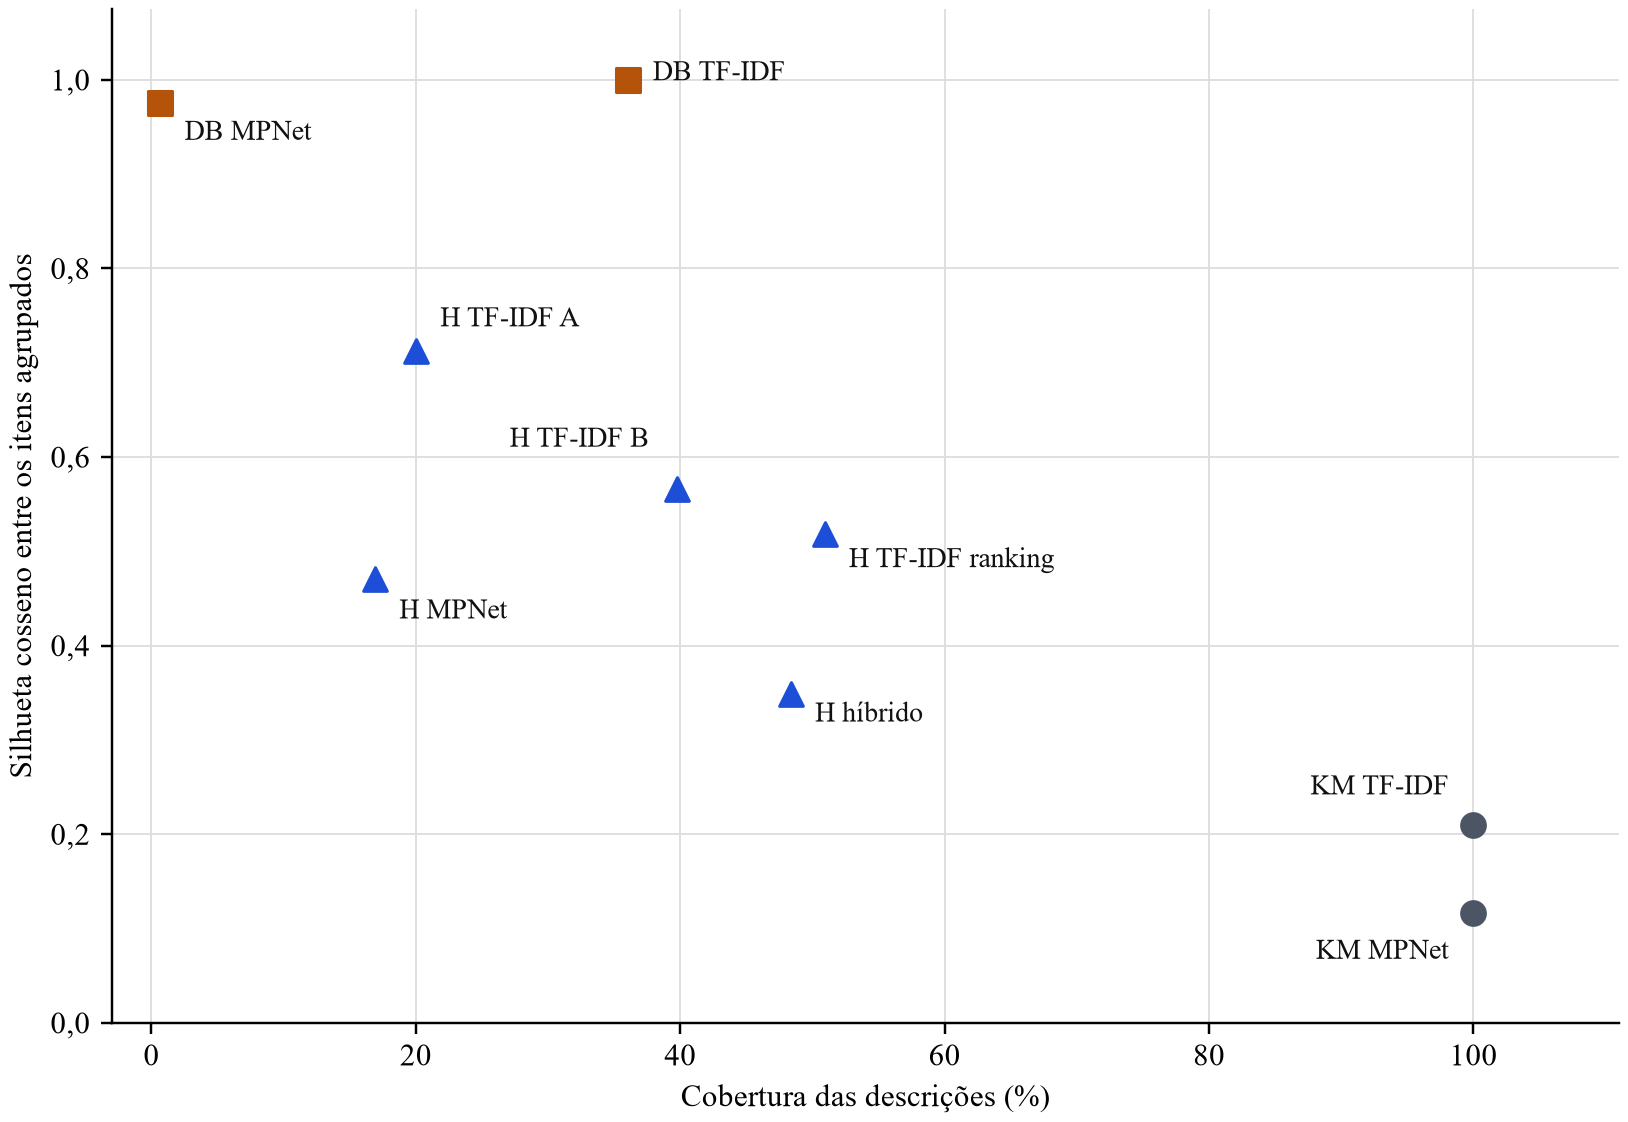
\includegraphics[width=0.85\linewidth]{images/cobertura-silhueta.png}
    \fonte{Elaborado pelo autor com base nos dados da Tabela~\ref{tab:indicadores}. KM: K-Means; DB: DBSCAN; H: HDBSCAN.}
\end{figure}

A Figura~\ref{fig:cobertura-silhueta} evidencia esse compromisso: as configurações DBSCAN destacadas alcançaram valores elevados de silhueta com cobertura restrita. As soluções HDBSCAN ocuparam posições intermediárias, com diferenças relevantes de cobertura e quantidade de grupos. O gráfico resume os indicadores e não representa uma ordenação definitiva da qualidade semântica dos agrupamentos.

\section{Resultados com K-Means}
\label{sec:res-kmeans}

Com TF-IDF, a maior silhueta observada foi 0,2099, na configuração de palavras com n-gramas de duas a cinco palavras, \texttt{min\_df} igual a dez e $k$ igual a 200. A pontuação composta foi 0,7037. Embora todas as descrições tenham recebido um cluster, o maior agrupamento reuniu 69,425\% da amostra, indicando forte concentração das atribuições.

Essa configuração também apresentou 10.796 vetores nulos, equivalentes a 53,98\% das descrições, e um vocabulário de 930 atributos. Portanto, a interpretação do resultado precisa considerar que mais da metade dos textos ficou sem atributos nessa representação. A combinação de n-gramas de pelo menos duas palavras com uma frequência mínima mais restritiva reduziu a informação disponível para distinguir parte das descrições. Como esses vetores são idênticos entre si, todos foram atribuídos ao mesmo centroide, o que explica a maior parte da concentração de 69,425\% observada no maior cluster.

As configurações seguintes do ranking TF-IDF utilizaram n-gramas de caracteres. Com \texttt{char\_wb} na faixa (4,10), \texttt{min\_df} igual a dez e $k$ igual a 200, a silhueta foi 0,1974. Com \texttt{char\_wb} na faixa (5,10), \texttt{min\_df} igual a cinco e o mesmo $k$, foi 0,1931. A maior silhueta, portanto, permaneceu próxima de 0,21 na grade avaliada.

Com os \textit{embeddings}, a maior silhueta foi 0,1165, também com $k$ igual a 200. O maior cluster representou 1,155\% das descrições, mostrando uma distribuição menos concentrada do que a configuração TF-IDF de maior pontuação. Essa distribuição, contudo, não foi acompanhada de maior silhueta. O resultado não sustentou a adoção do K-Means como solução suficiente para o objetivo do trabalho e motivou a continuidade da investigação com métodos baseados em densidade.

As Figuras~\ref{fig:tsne-kmeans-tfidf} e~\ref{fig:tsne-kmeans-mpnet} apresentam as projeções t-SNE das configurações K-Means destacadas. Na representação TF-IDF, os vetores nulos aparecem concentrados em uma única região, em forma de anel, e com a mesma cor, pois foram atribuídos ao mesmo cluster. Com os \textit{embeddings}, as descrições se distribuem de forma mais contínua, com regiões de maior densidade, mas sem separação nítida entre muitos dos grupos.

\begin{figure}[htbp]
    \caption{Projeção t-SNE da configuração TF-IDF com K-Means destacada (palavras de duas a cinco, $k$ igual a 200)}
    \label{fig:tsne-kmeans-tfidf}
    \centering
    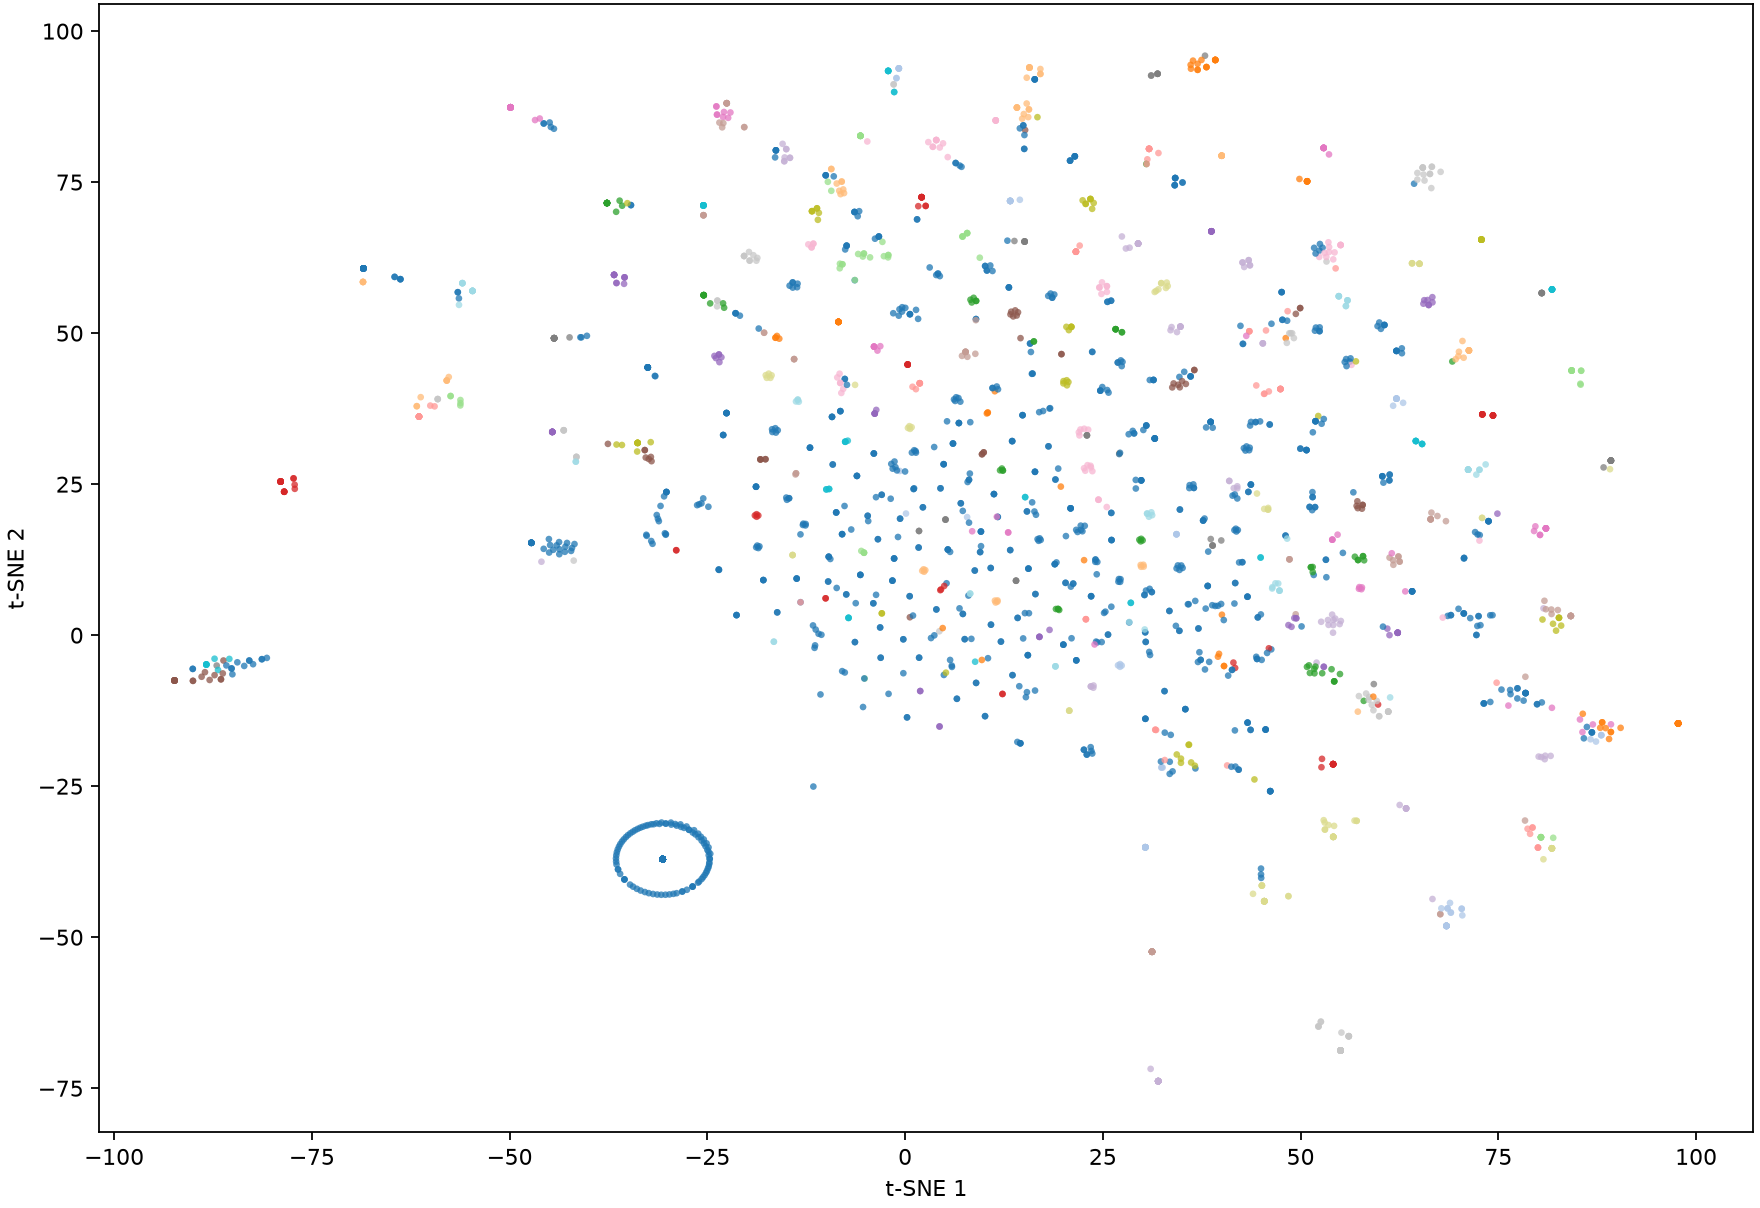
\includegraphics[width=0.85\linewidth]{images/tsne-kmeans-tfidf.png}
    \fonte{Elaborado pelo autor. Projeção t-SNE de uma amostra de 5.000 descrições; as cores se repetem a cada 20 clusters. As quantidades visíveis na projeção podem diferir das da Tabela~\ref{tab:indicadores}, calculadas sobre 20.000 descrições.}
\end{figure}

\begin{figure}[htbp]
    \caption{Projeção t-SNE da configuração MPNet com K-Means destacada ($k$ igual a 200)}
    \label{fig:tsne-kmeans-mpnet}
    \centering
    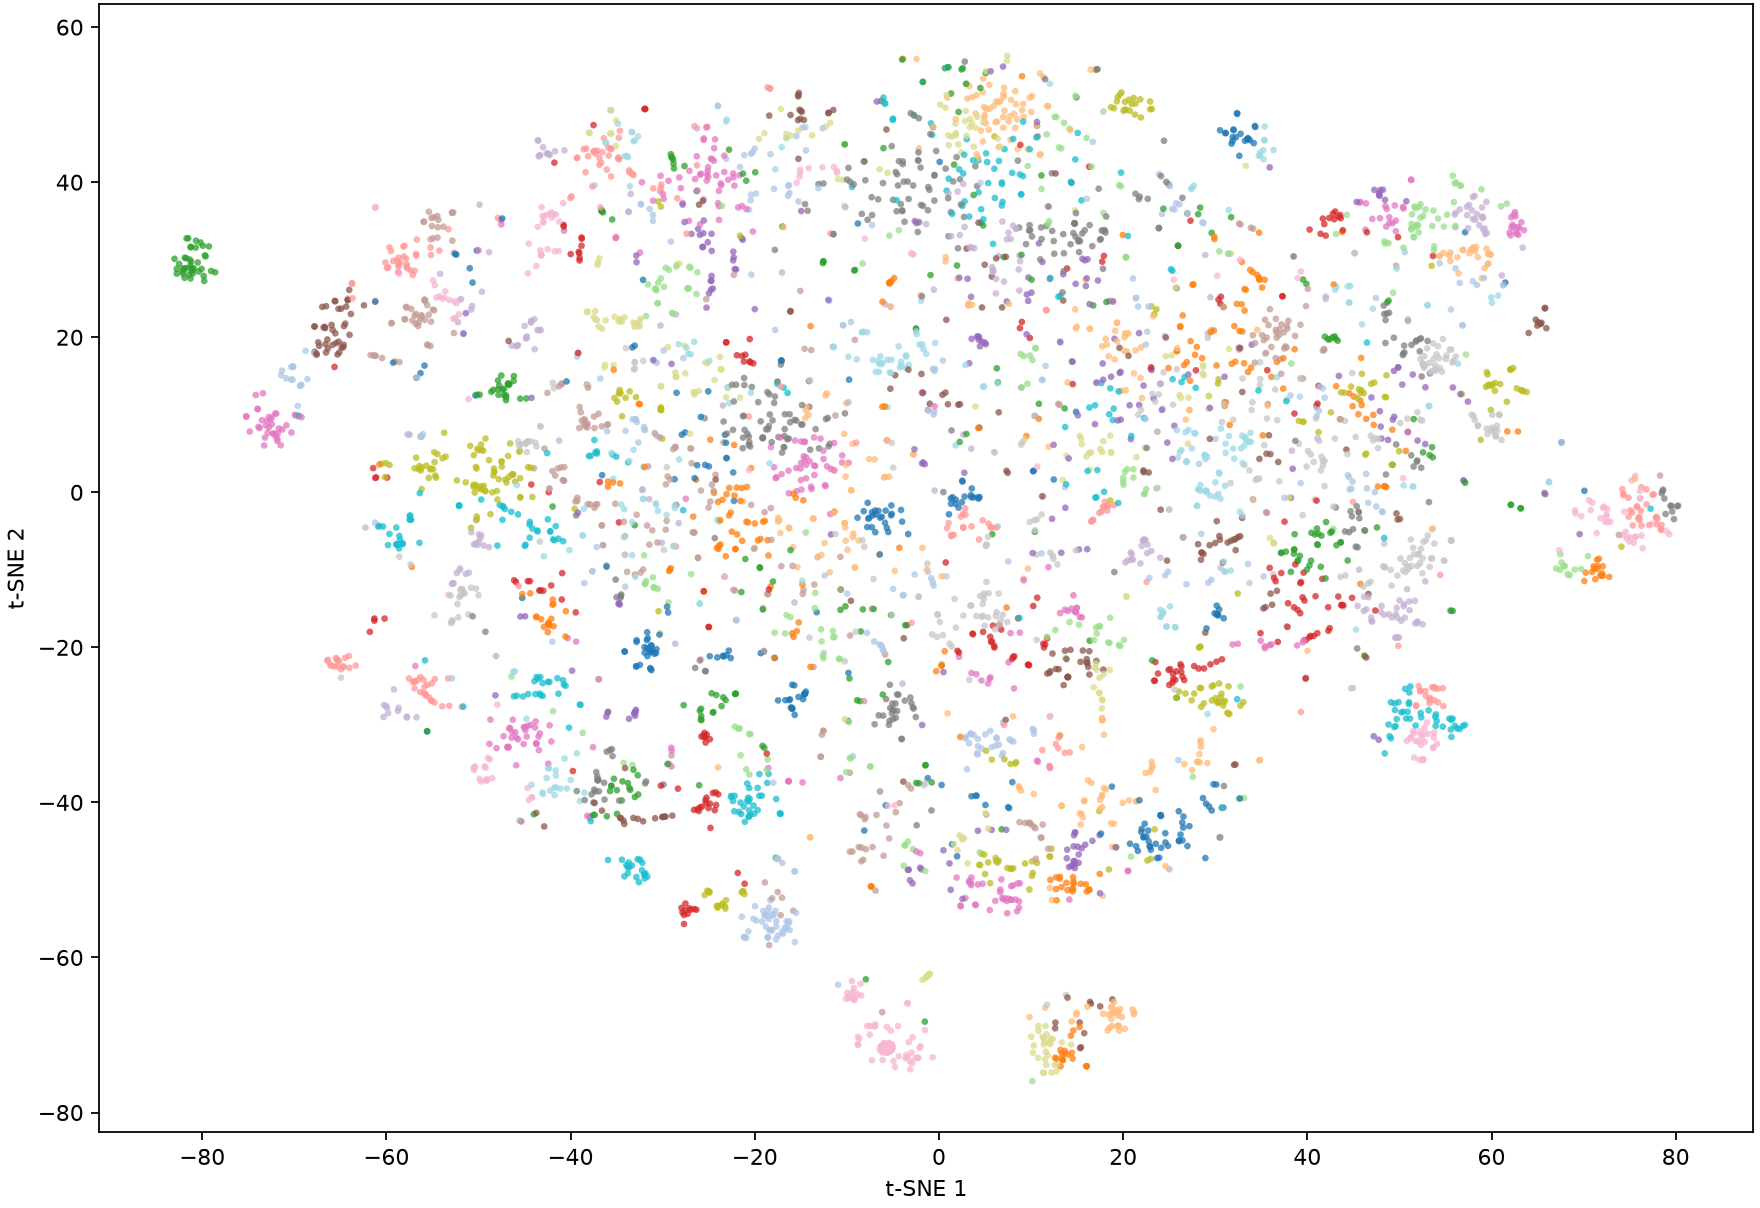
\includegraphics[width=0.85\linewidth]{images/tsne-kmeans-mpnet.png}
    \fonte{Elaborado pelo autor. Projeção t-SNE de uma amostra de 5.000 descrições; as cores se repetem a cada 20 clusters. As quantidades visíveis na projeção podem diferir das da Tabela~\ref{tab:indicadores}, calculadas sobre 20.000 descrições.}
\end{figure}

\section{Resultados com DBSCAN}
\label{sec:res-dbscan}

No TF-IDF com DBSCAN, a primeira posição do ranking utilizou n-gramas de duas a cinco palavras, \texttt{min\_df} igual a dez, \texttt{eps} igual a 0,025 e \texttt{min\_samples} igual a três. Foram formados 734 clusters, com silhueta de 0,9996. Entretanto, 12.783 descrições foram identificadas como ruído, correspondendo a 63,915\% da amostra. A silhueta descreveu somente as 7.217 observações agrupadas.

A mesma representação apresentou 10.796 vetores nulos. A silhueta elevada, nesse cenário, indica separação dos grupos no espaço dos atributos retidos, mas não demonstra que a representação conseguiu organizar semanticamente toda a diversidade textual. O percentual de ruído e a quantidade de descrições sem atributos limitaram a utilidade desse resultado para uma categorização com maior cobertura.

Com MPNet e DBSCAN, a primeira configuração do ranking utilizou \texttt{eps} igual a 0,01 e \texttt{min\_samples} igual a cinco. Foram identificados onze clusters e silhueta de 0,9753. Porém, apenas 133 descrições receberam cluster, enquanto 19.867 ficaram como ruído. A cobertura foi de 0,665\%, e a proporção de ruído atingiu 99,335\%.

Assim, o ganho de silhueta em relação ao K-Means foi acompanhado de uma redução importante da cobertura nas configurações destacadas. O caso dos \textit{embeddings} demonstra que atender ao mínimo de dez clusters não basta para tornar uma solução adequada: mesmo com onze grupos e silhueta elevada, quase todas as descrições ficaram sem atribuição. Esses resultados reforçaram a necessidade de considerar os indicadores conjuntamente.

As Figuras~\ref{fig:tsne-dbscan-tfidf} e~\ref{fig:tsne-dbscan-mpnet} mostram as projeções das configurações DBSCAN destacadas, com o ruído representado em cinza. Com TF-IDF, os clusters aparecem como pequenos conjuntos de pontos sobrepostos, compatíveis com grupos de descrições muito semelhantes, enquanto o anel dos vetores nulos permanece como ruído. Com os \textit{embeddings}, quase toda a amostra permanece em cinza, o que ilustra a cobertura de 0,665\%.

\begin{figure}[htbp]
    \caption{Projeção t-SNE da configuração TF-IDF com DBSCAN destacada (palavras de duas a cinco, \texttt{eps} igual a 0,025 e \texttt{min\_samples} igual a três)}
    \label{fig:tsne-dbscan-tfidf}
    \centering
    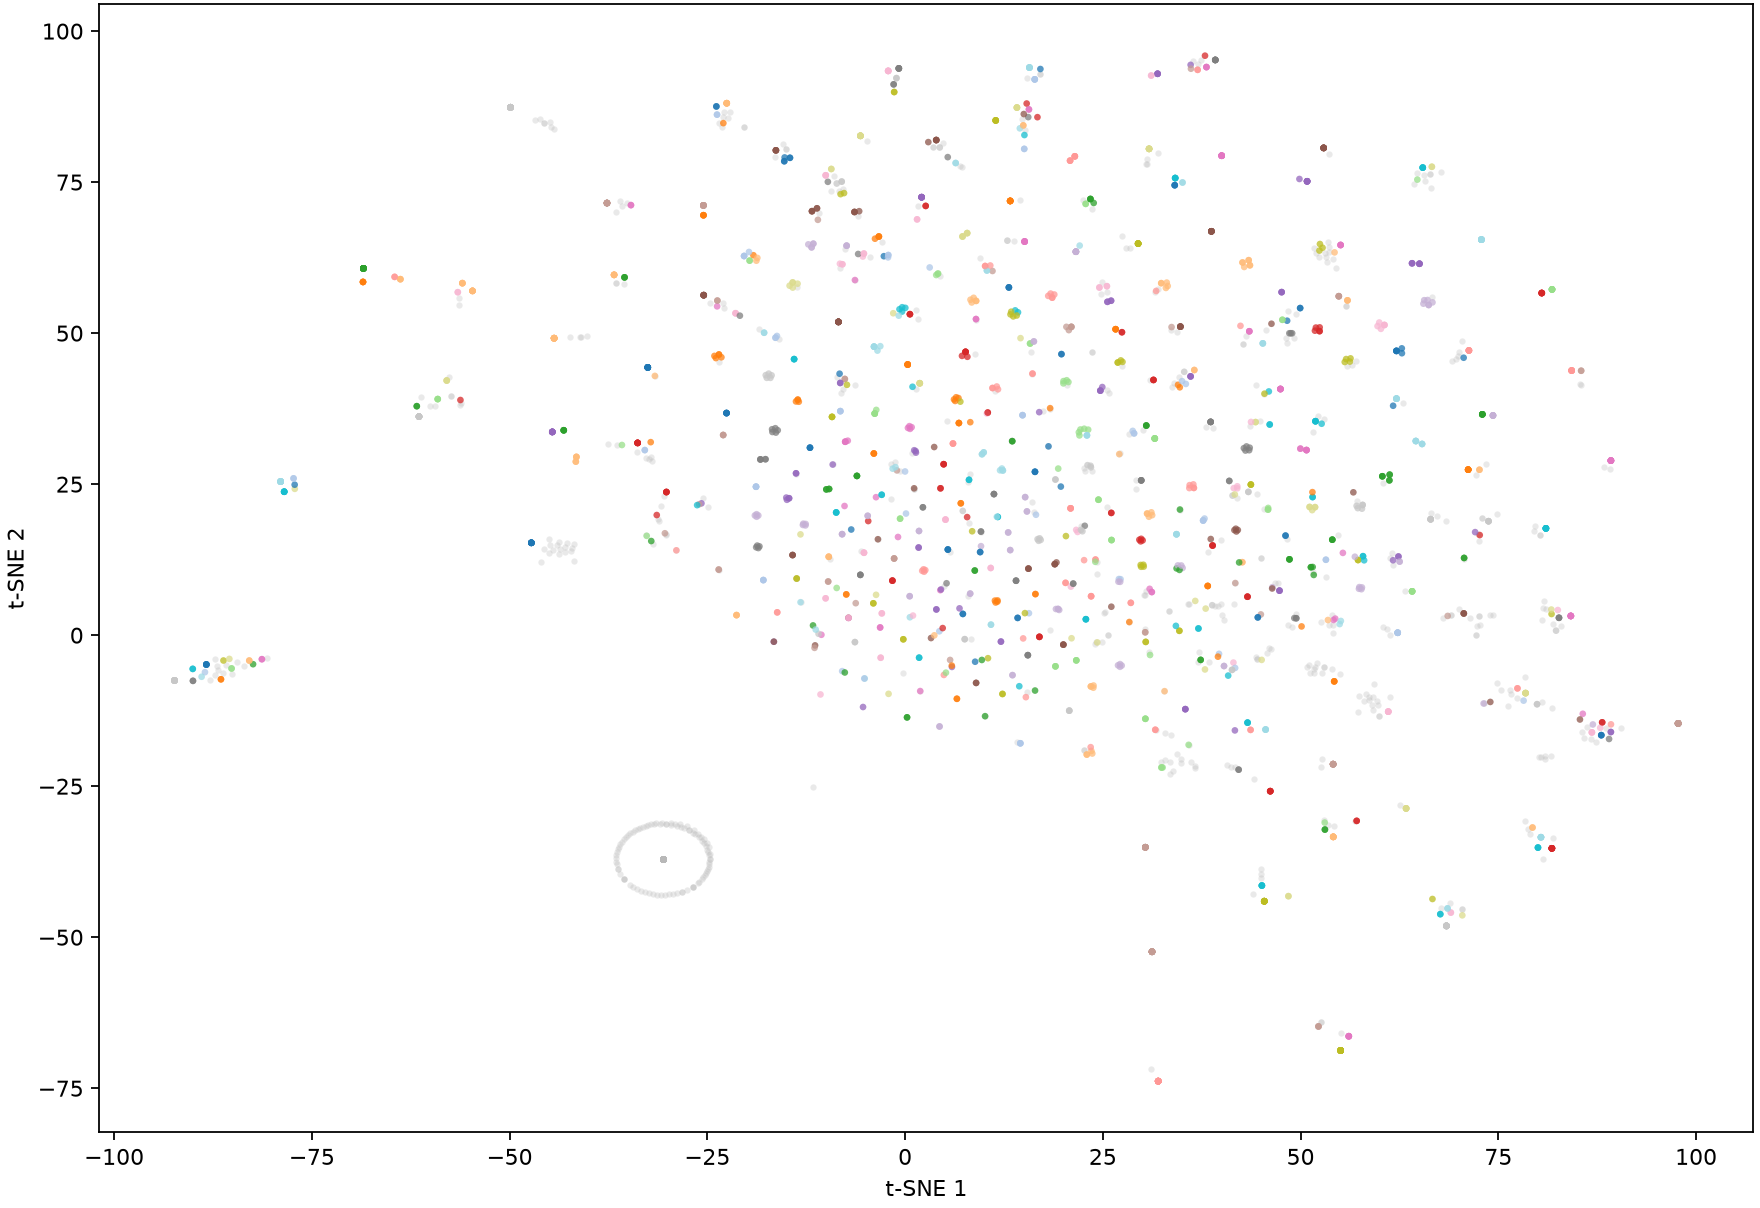
\includegraphics[width=0.85\linewidth]{images/tsne-dbscan-tfidf.png}
    \fonte{Elaborado pelo autor. Projeção t-SNE de uma amostra de 5.000 descrições; ruído em cinza; as cores se repetem a cada 20 clusters. As quantidades visíveis na projeção podem diferir das da Tabela~\ref{tab:indicadores}, calculadas sobre 20.000 descrições.}
\end{figure}

\begin{figure}[htbp]
    \caption{Projeção t-SNE da configuração MPNet com DBSCAN destacada (\texttt{eps} igual a 0,01 e \texttt{min\_samples} igual a cinco)}
    \label{fig:tsne-dbscan-mpnet}
    \centering
    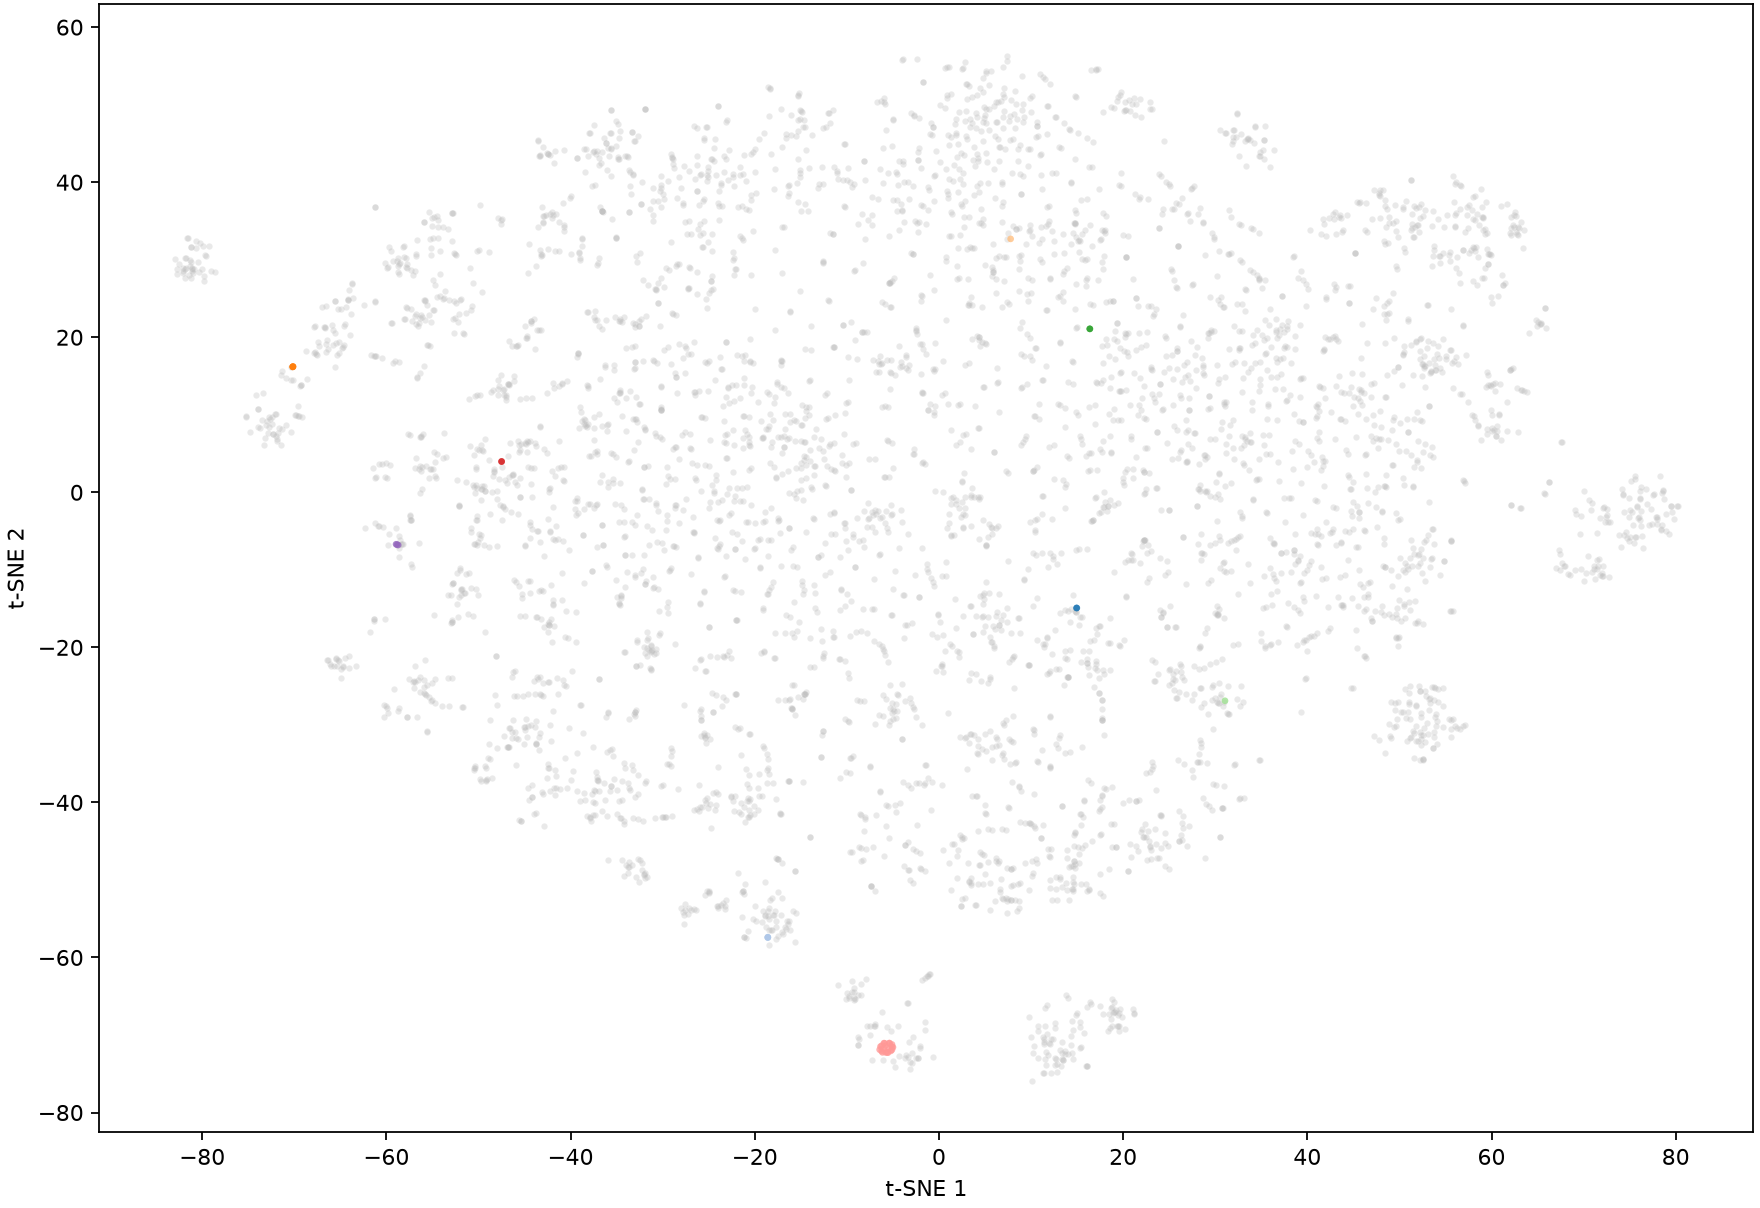
\includegraphics[width=0.85\linewidth]{images/tsne-dbscan-mpnet.png}
    \fonte{Elaborado pelo autor. Projeção t-SNE de uma amostra de 5.000 descrições; ruído em cinza; as cores se repetem a cada 20 clusters. As quantidades visíveis na projeção podem diferir das da Tabela~\ref{tab:indicadores}, calculadas sobre 20.000 descrições.}
\end{figure}

\section{Resultados com HDBSCAN}
\label{sec:res-hdbscan}

\subsection{TF-IDF e configurações selecionadas para aprofundamento}

Com TF-IDF, a primeira configuração do ranking HDBSCAN utilizou \texttt{char\_wb} na faixa (5,10), \texttt{min\_df} igual a dez, \texttt{min\_cluster\_size} igual a cinco e \texttt{min\_samples} padrão. Foram obtidos 736 clusters, silhueta de 0,5189 e ruído de 49,085\%. A segunda configuração apresentou os mesmos indicadores ao explicitar \texttt{min\_samples} igual a cinco. Como o valor padrão assume o tamanho mínimo do cluster, as duas linhas correspondem aos mesmos parâmetros efetivos.

Apesar da posição no ranking, a formação de mais de setecentos grupos foi considerada excessivamente fragmentada pelo autor para a continuidade da interpretação. Foram destacadas duas alternativas com menor quantidade de clusters, denominadas A e B nesta apresentação.

A candidata A utilizou n-gramas de palavras na faixa (2,5), \texttt{min\_df} igual a dez, \texttt{min\_cluster\_size} igual a vinte e \texttt{min\_samples} padrão, equivalente a vinte. Essa configuração formou 101 clusters e apresentou silhueta de 0,7127, com pontuação composta de 0,6923. Foram agrupadas 4.001 descrições, correspondendo à cobertura de 20,005\%, enquanto 79,995\% permaneceram como ruído.

A candidata B utilizou \texttt{char\_wb} na faixa (5,10), \texttt{min\_df} igual a dez, \texttt{min\_cluster\_size} igual a cinco e \texttt{min\_samples} igual a dez. Foram identificados 381 clusters, com silhueta de 0,5656 e pontuação de 0,6865. Essa alternativa agrupou 7.947 descrições, alcançando cobertura de 39,735\%, com 60,265\% de ruído. A Tabela~\ref{tab:candidatas} compara as representações das duas candidatas.

\begin{table}[htbp]
    \caption{Características das representações das candidatas HDBSCAN}
    \label{tab:candidatas}
    \centering
    \small
    \begin{tabularx}{\textwidth}{lXrr}
        \hline
        \textbf{Candidata} & \textbf{Representação} & \textbf{Atributos} & \textbf{Vetores nulos}\\
        \hline
        A & Palavras de duas a cinco & 930 & 10.796 (53,98\%)\\
        B & Caracteres de cinco a dez & 18.111 & 47 (0,235\%)\\
        \hline
    \end{tabularx}
    \fonte{Elaborado pelo autor com base nas métricas do notebook 74.}
\end{table}

As duas candidatas expressam compromissos diferentes. A alternativa A apresentou maior silhueta e menor quantidade de clusters, com cobertura mais restrita. A alternativa B incluiu uma parcela maior das descrições e produziu menos vetores nulos, embora tenha formado mais grupos e apresentado silhueta inferior. A diferença de representação da Tabela~\ref{tab:candidatas} é relevante para avaliar se os grupos encontrados resultam de informação textual suficiente.

Essas configurações foram consideradas de interesse por produzirem quantidades de agrupamentos mais viáveis para aprofundamento do que as duas primeiras posições do ranking. Essa seleção é provisória: a maior silhueta da candidata A não elimina a limitação de seus vetores nulos e de sua cobertura, e a adequação dos 381 clusters da candidata B ainda depende da inspeção de seu conteúdo.

As Figuras~\ref{fig:tsne-hdbscan-a} e~\ref{fig:tsne-hdbscan-b} apresentam as projeções das candidatas A e B. Na candidata A, o anel formado pelos vetores nulos contém pontos atribuídos a clusters. A verificação das atribuições dessa configuração mostrou que 316 descrições sem atributos receberam cluster. No maior desses grupos, 264 dos 337 itens não possuíam atributos e reuniam produtos sem relação entre si, como frutas, fitas adesivas e álcool. Na candidata B, os grupos se distribuem por toda a projeção, e os vetores nulos são raros.

\begin{figure}[htbp]
    \caption{Projeção t-SNE da candidata A (TF-IDF de palavras com HDBSCAN)}
    \label{fig:tsne-hdbscan-a}
    \centering
    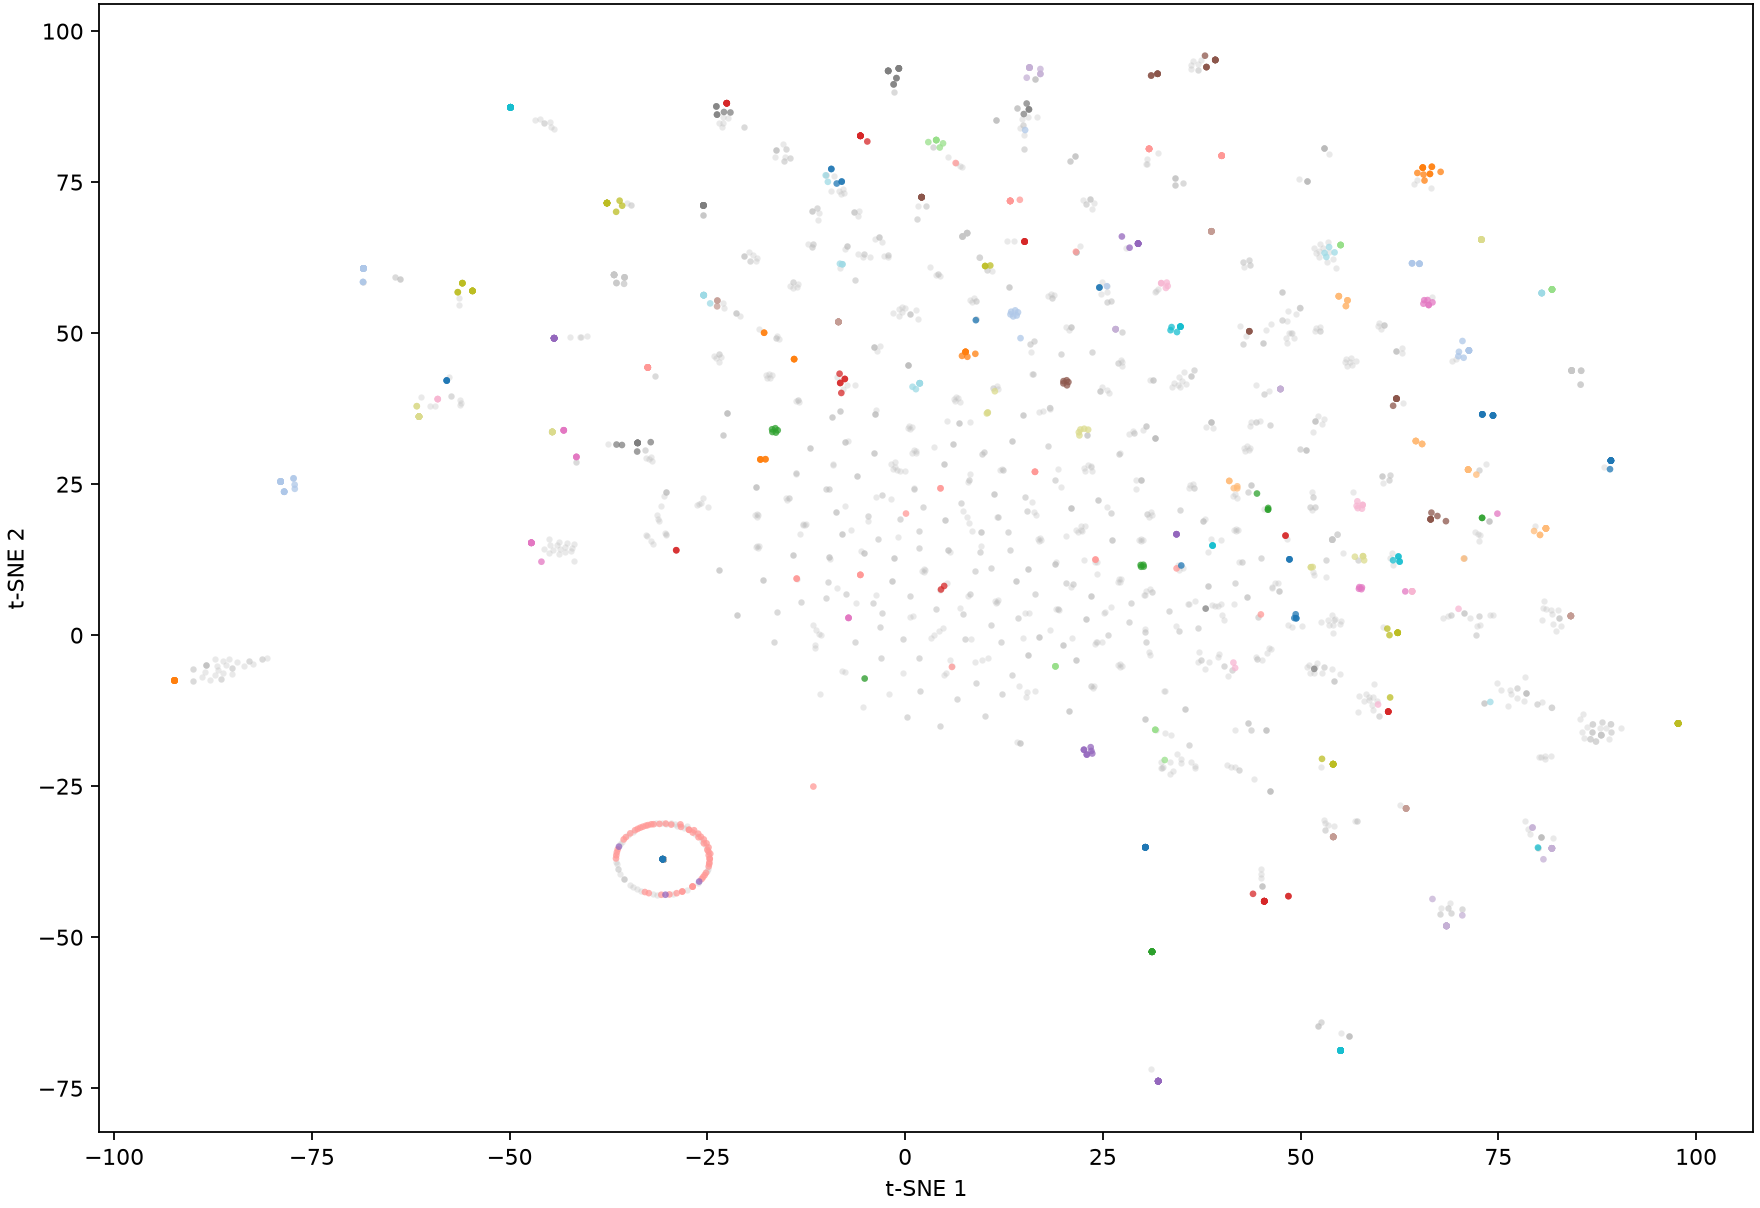
\includegraphics[width=0.85\linewidth]{images/tsne-hdbscan-candidata-a.png}
    \fonte{Elaborado pelo autor. Projeção t-SNE de uma amostra de 5.000 descrições; ruído em cinza; as cores se repetem a cada 20 clusters. As quantidades visíveis na projeção podem diferir das da Tabela~\ref{tab:indicadores}, calculadas sobre 20.000 descrições.}
\end{figure}

\begin{figure}[htbp]
    \caption{Projeção t-SNE da candidata B (TF-IDF de caracteres com HDBSCAN)}
    \label{fig:tsne-hdbscan-b}
    \centering
    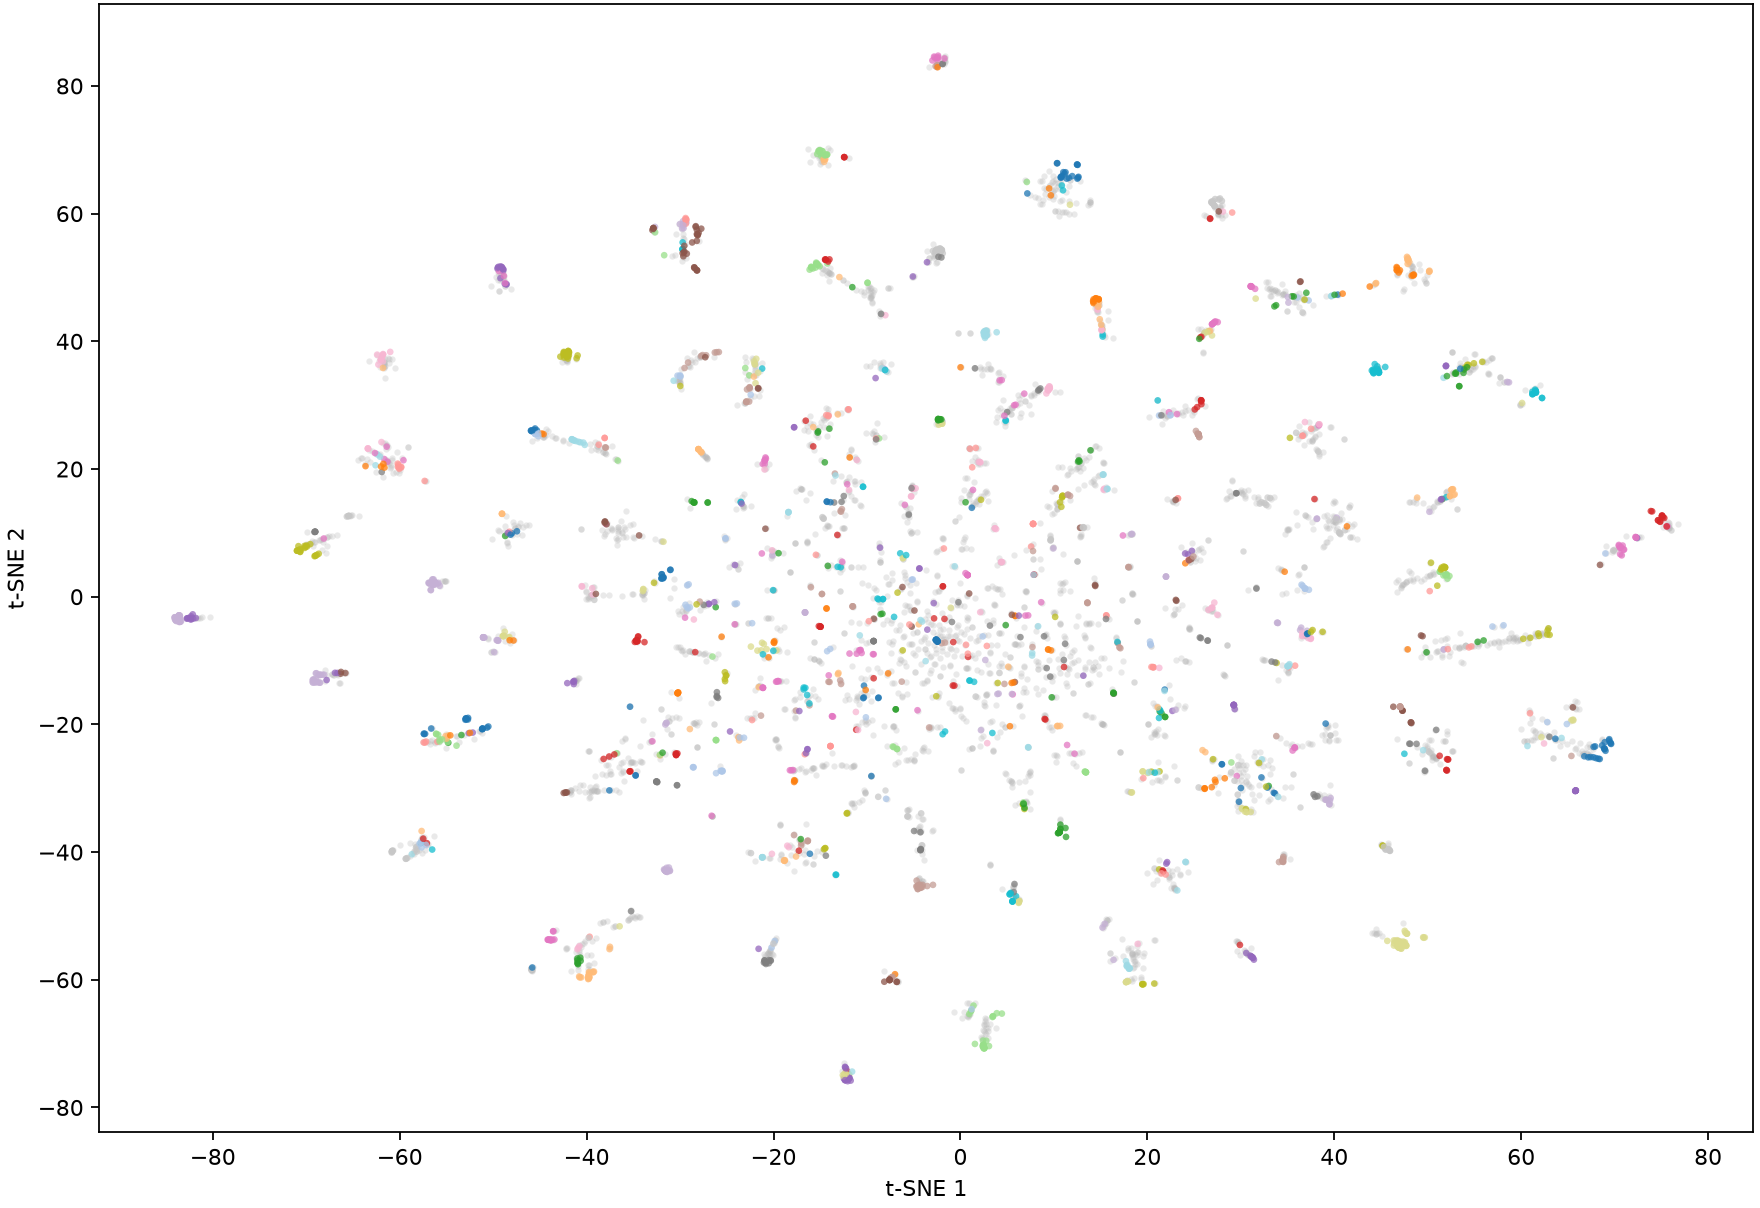
\includegraphics[width=0.85\linewidth]{images/tsne-hdbscan-candidata-b.png}
    \fonte{Elaborado pelo autor. Projeção t-SNE de uma amostra de 5.000 descrições; ruído em cinza; as cores se repetem a cada 20 clusters. As quantidades visíveis na projeção podem diferir das da Tabela~\ref{tab:indicadores}, calculadas sobre 20.000 descrições.}
\end{figure}

\subsection{Embeddings MPNet}
\label{sec:res-hdbscan-mpnet}

Com MPNet e HDBSCAN, a primeira configuração do ranking utilizou \texttt{min\_cluster\_size} igual a cinco e \texttt{min\_samples} igual a dez. Foram identificados 123 clusters, com silhueta de 0,4710 e pontuação de 0,5939. A proporção de ruído foi 83,095\%, e 3.381 descrições foram agrupadas, resultando em cobertura de 16,905\%.

Em relação às duas candidatas TF-IDF destacadas, essa configuração apresentou menor silhueta e menor cobertura. Na inspeção exploratória realizada no Excel, entretanto, o autor observou agrupamentos percebidos como semanticamente mais coesos com os \textit{embeddings}. Essa percepção sugere que as métricas geométricas não esgotam a interpretação do conteúdo dos grupos.

A observação qualitativa ainda precisa ser aprofundada e documentada com exemplos e critérios consistentes de julgamento. Ela é tratada como indício exploratório, sem demonstrar superioridade semântica geral do modelo ou correção das categorias em descrições não utilizadas no agrupamento.

A Figura~\ref{fig:tsne-hdbscan-mpnet} apresenta a projeção da configuração MPNet destacada. Os grupos aparecem como regiões compactas, distribuídas por toda a projeção, enquanto a maior parte das descrições permanece como ruído.

\begin{figure}[htbp]
    \caption{Projeção t-SNE da configuração MPNet com HDBSCAN destacada (\texttt{min\_cluster\_size} igual a cinco e \texttt{min\_samples} igual a dez)}
    \label{fig:tsne-hdbscan-mpnet}
    \centering
    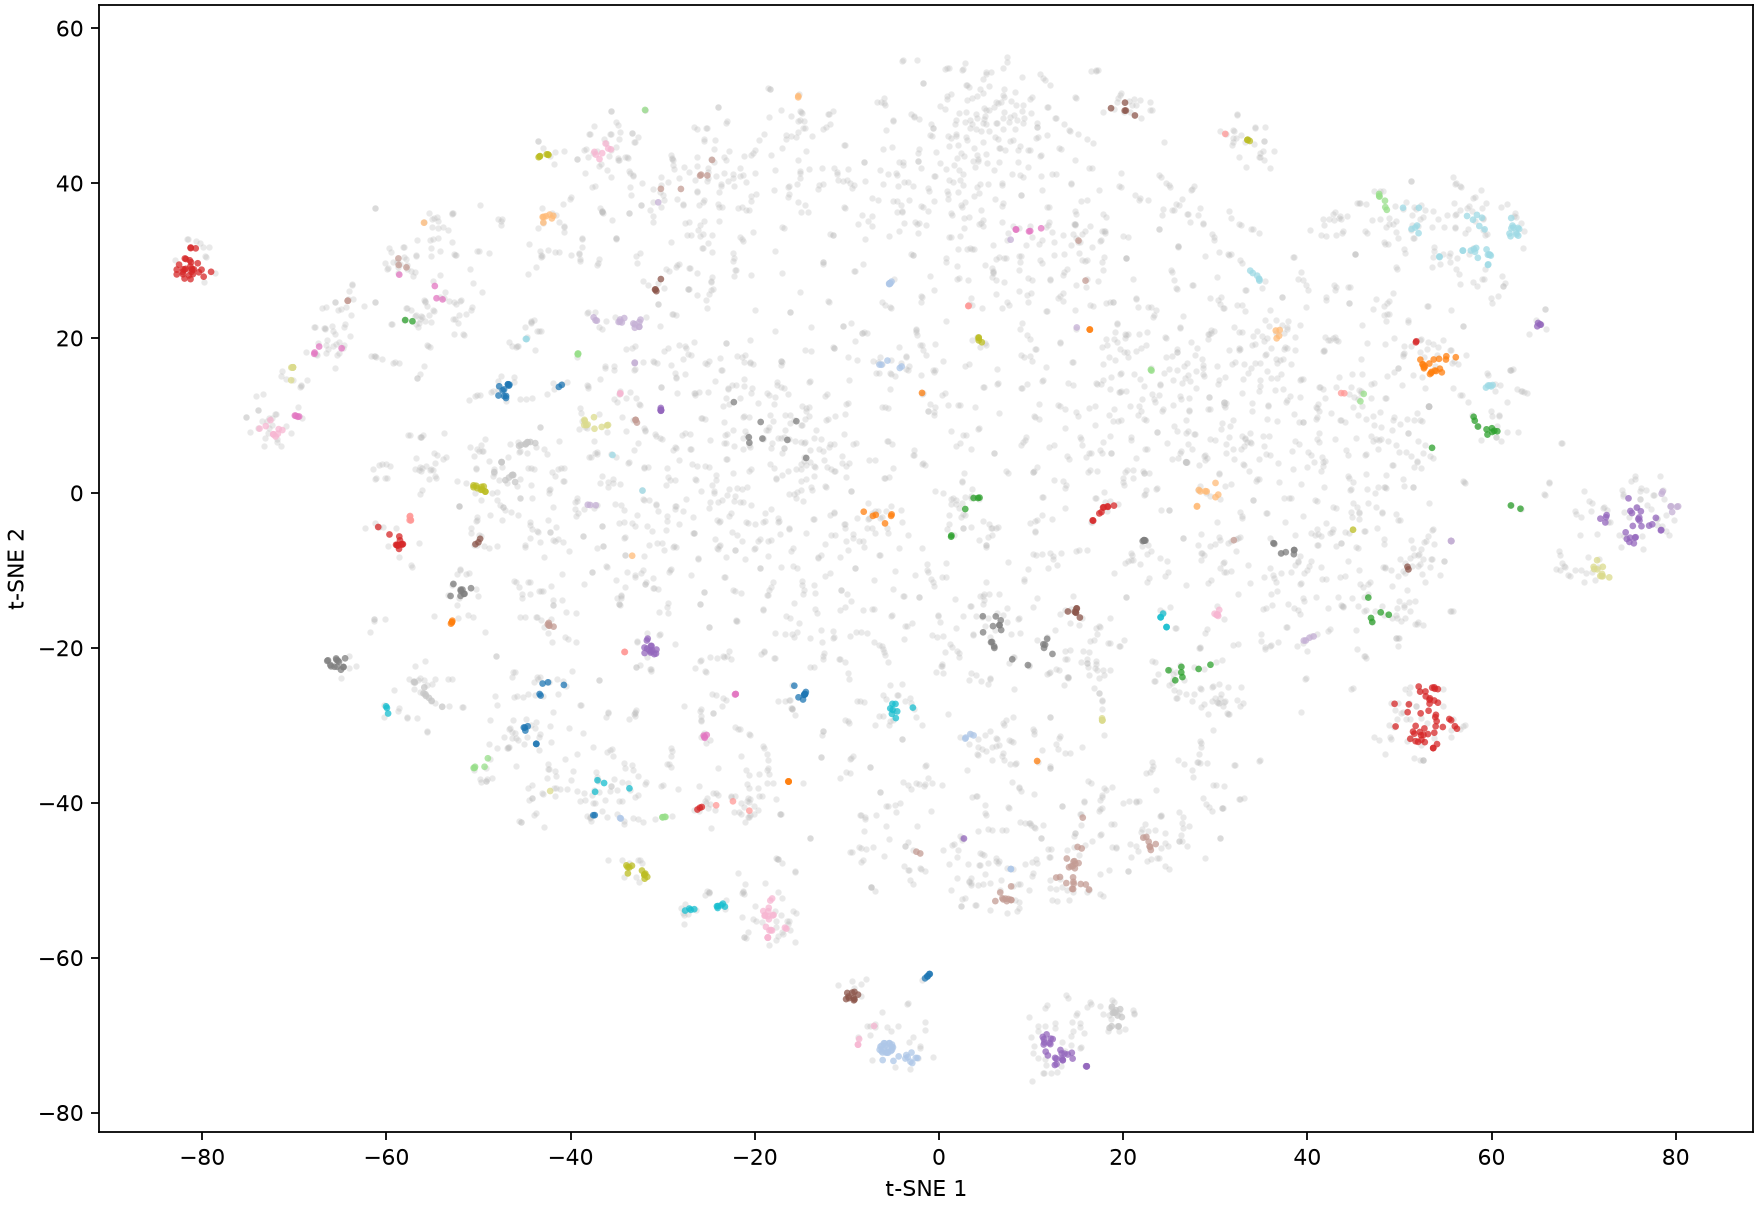
\includegraphics[width=0.85\linewidth]{images/tsne-hdbscan-mpnet.png}
    \fonte{Elaborado pelo autor. Projeção t-SNE de uma amostra de 5.000 descrições; ruído em cinza; as cores se repetem a cada 20 clusters. As quantidades visíveis na projeção podem diferir das da Tabela~\ref{tab:indicadores}, calculadas sobre 20.000 descrições.}
\end{figure}

\subsection{Representação híbrida}

Na representação híbrida com $\alpha$ igual a 0,2, a primeira posição do ranking utilizou TF-IDF de palavras na faixa (2,5), \texttt{min\_df} igual a cinco, \texttt{min\_cluster\_size} igual a cinco e \texttt{min\_samples} igual a dois. Essa configuração formou 982 clusters, com silhueta de 0,3487 e pontuação de 0,6266. Foram agrupadas 9.671 descrições, correspondendo a 48,355\% da amostra; a proporção de ruído foi 51,645\%.

A combinação incluiu uma parcela maior de descrições do que a configuração MPNet destacada, mas apresentou silhueta inferior. Em comparação com a primeira configuração TF-IDF com HDBSCAN, apresentou tanto menor silhueta quanto menor cobertura, além de maior quantidade de clusters. A representação híbrida, portanto, não resultou em melhora simultânea desses indicadores nas configurações que lideraram os respectivos rankings.

O resultado também mostra que a combinação das representações não resolveu automaticamente a fragmentação observada. A contribuição semântica dos \textit{embeddings} na solução híbrida ainda depende de uma análise do conteúdo dos grupos, que não foi concluída nesta etapa.

\section{Inspeção dos agrupamentos e testes do protótipo}
\label{sec:res-inspecao}

Os arquivos de atribuições permitiram consultar as descrições associadas a cada cluster e organizar sua visualização em tabelas dinâmicas do Excel. Essa inspeção apoiou a seleção de configurações com quantidade de grupos considerada mais adequada ao aprofundamento da análise e possibilitou a observação exploratória de diferenças de coerência semântica entre as representações.

A revisão manual descrita na Seção~\ref{sec:criterios} sistematizou essa inspeção. A Tabela~\ref{tab:revisao} apresenta, para cada configuração, a silhueta, a cobertura, a classificação dos clusters sorteados e a estimativa da parcela das descrições em clusters coerentes.

\begin{table}[htbp]
    \caption{Resultado da revisão manual dos clusters}
    \label{tab:revisao}
    \centering
    \small
    \begin{tabularx}{\textwidth}{Xrrrrrr}
        \hline
        \textbf{Configuração} & \textbf{Silhueta} & \textbf{Cobertura (\%)} & \textbf{Coerentes} & \textbf{Parciais} & \textbf{Incoerentes} & \textbf{Descrições em clusters coerentes (\%)}\\
        \hline
        TF-IDF e K-Means & 0,2099 & 100,000 & 17 & 2 & 2 & 24,4\\
        MPNet e K-Means & 0,1165 & 100,000 & 6 & 6 & 9 & 19,5\\
        TF-IDF e DBSCAN & 0,9996 & 36,085 & 21 & 0 & 0 & 36,1\\
        MPNet e DBSCAN & 0,9753 & 0,665 & 11 & 0 & 0 & 0,7\\
        TF-IDF e HDBSCAN (primeira do ranking) & 0,5189 & 50,915 & 20 & 0 & 1 & 48,8\\
        TF-IDF e HDBSCAN (candidata A) & 0,7127 & 20,005 & 17 & 4 & 0 & 17,4\\
        TF-IDF e HDBSCAN (candidata B) & 0,5656 & 39,735 & 19 & 2 & 0 & 36,4\\
        MPNet e HDBSCAN & 0,4710 & 16,905 & 18 & 1 & 2 & 15,2\\
        TF-IDF e MPNet com HDBSCAN & 0,3487 & 48,355 & 18 & 3 & 0 & 42,7\\
        \hline
    \end{tabularx}
    \fonte{Elaborado pelo autor com base na revisão manual da amostra de clusters e nos dados da Tabela~\ref{tab:indicadores}. Nota: as colunas Coerentes, Parciais e Incoerentes indicam quantidades de clusters entre os 21 sorteados em cada configuração, ou entre os 11 clusters de MPNet e DBSCAN. A última coluna estima a parcela das 20.000 descrições que pertence a clusters avaliados como coerentes.}
\end{table}

Nas configurações K-Means, a revisão confirmou a limitação indicada pelas métricas. Com TF-IDF, 17 dos 21 clusters sorteados foram considerados coerentes, mas o maior cluster, que não integrou a amostra, reuniu 13.885 descrições, incluindo todas as 10.796 sem atributos TF-IDF. Esse grupo foi classificado como incoerente, e a parcela estimada de descrições em clusters coerentes foi de 24,4\%. Com \textit{embeddings}, apenas 6 dos 21 clusters foram considerados coerentes, e os clusters maiores reuniram produtos de tipos variados, resultando em 19,5\%, a menor estimativa entre as configurações com cobertura completa.

As duas configurações DBSCAN tiveram todos os clusters sorteados avaliados como coerentes, o que é compatível com suas silhuetas próximas de um. A baixa cobertura, contudo, limitou a parcela das descrições em clusters coerentes a 36,1\% com TF-IDF e 0,7\% com MPNet. Além disso, nove dos onze clusters de MPNet com DBSCAN reuniram variações de uma mesma mercadoria, diferenciadas apenas por lote, quantidade ou dados do documento fiscal, o que constitui uma coerência pouco informativa para a categorização.

Nas configurações HDBSCAN, entre 17 e 20 dos 21 clusters sorteados foram avaliados como coerentes. As maiores parcelas de descrições em clusters coerentes foram observadas na primeira configuração TF-IDF do ranking (48,8\%) e na representação híbrida (42,7\%), justamente as soluções com maior quantidade de clusters. Entre as candidatas, a B apresentou 19 clusters coerentes, contra 17 da A, e maior parcela estimada (36,4\% e 17,4\%, respectivamente). A configuração MPNet apresentou 18 clusters coerentes, mas sua cobertura limitou a estimativa a 15,2\%.

Na amostra avaliada, a percepção exploratória de maior coesão dos agrupamentos com \textit{embeddings}, registrada na Seção~\ref{sec:res-hdbscan-mpnet}, não se confirmou de forma clara: a quantidade de clusters coerentes de MPNet com HDBSCAN ficou entre as das candidatas A e B. De modo geral, a silhueta isolada não indicou qual configuração organiza mais descrições em grupos coerentes. A coerência dos grupos formados e a cobertura precisam ser consideradas em conjunto.

Até esta etapa, não foi estabelecido um conjunto consolidado de categorias específicas nem um mapeamento definitivo entre identificadores de cluster e nomes de categorias. A reunião de clusters semelhantes em uma mesma categoria, a análise das atribuições individuais e o tratamento de descrições ambíguas permanecem em desenvolvimento.

O notebook de consulta possibilitou testar manualmente algumas descrições e recuperar exemplos de um agrupamento. Esses testes demonstram o funcionamento parcial do mecanismo de consulta, mas não constituem uma avaliação da categorização. Também foi registrada uma limitação para entradas curtas: a descrição ``pao'', consultada com um vocabulário baseado em n-gramas de pelo menos duas palavras, não produziu atributos TF-IDF válidos. Nesse caso, a execução apresentou uma mensagem de erro, sem atribuir um grupo.

A reserva de 300 descrições não foi avaliada com rótulos humanos. Consequentemente, ainda não há resultados de acurácia, precisão, revocação ou F1 para a categorização de novas entradas. As métricas de agrupamento apresentadas neste capítulo não devem ser interpretadas como substitutas dessa avaliação.

\section{Discussão dos resultados e limitações}
\label{sec:discussao}

Os experimentos mostraram que a escolha do algoritmo precisa considerar mais do que o maior valor de silhueta. O K-Means atribuiu todas as descrições, mas os melhores valores observados ficaram próximos de 0,21 com TF-IDF e 0,12 com \textit{embeddings}. O DBSCAN identificou grupos com silhueta elevada nas configurações destacadas, ao custo de deixar uma parcela importante dos dados sem agrupamento.

O HDBSCAN ofereceu alternativas de interesse para prosseguir com a investigação, especialmente as soluções TF-IDF com 101 e 381 clusters. Essa avaliação se apoia no compromisso observado entre separação, cobertura e quantidade de grupos, além da inspeção exploratória. Ela não estabelece superioridade em todos os indicadores, e as proporções de ruído dessas alternativas continuam limitando seu alcance.

A presença de vetores nulos constitui uma limitação relevante dos resultados baseados em TF-IDF. Na candidata A, mais da metade das descrições não foi representada por atributos. A revisão do conteúdo dos clusters e do ruído deverá considerar esse diagnóstico para distinguir dificuldades do agrupamento de perdas de informação decorrentes do vocabulário.

A comparação foi realizada sobre uma única amostra e uma única semente de seleção. As dez inicializações do K-Means integram o ajuste de cada configuração, mas não equivalem a repetir todo o protocolo em diferentes amostras. Não foi estimada a variabilidade dos resultados decorrente dessas escolhas. Além disso, a consolidação remove duplicatas exatas do texto tratado, mas não impede que descrições muito semelhantes representem produtos relacionados em diferentes partições.

Outra limitação decorre da origem dos dados. O filtro por NCM aproxima os tipos de mercadorias do domínio pretendido, porém mantém a população de aquisições públicas da fonte. A generalização para descrições de compras de consumidores em supermercados exige avaliação específica em dados desse contexto.

A revisão manual também apresenta limitações. Ela foi realizada por um único avaliador, sem medida de concordância entre avaliadores, e sobre uma amostra de até 21 clusters por configuração, de modo que um único cluster grande pode alterar de forma sensível a estimativa da parcela de descrições em clusters coerentes. Parte das classificações preliminares foi elaborada com apoio de inteligência artificial, o que exigiu a conferência integral pelo autor, mas pode ter influenciado a aplicação dos critérios. Além disso, os critérios verificam se as descrições apresentadas correspondem a um mesmo tipo de produto, mas não avaliam se o nível de agregação é adequado às categorias comerciais pretendidas, nem se grupos distintos deveriam ser reunidos em uma mesma categoria.

Os resultados disponíveis sustentam uma análise dos agrupamentos e a seleção de alternativas para revisão mais detalhada. A validação das categorias comerciais e a avaliação do protótipo ainda precisam ser realizadas. Assim, a contribuição demonstrada até esta etapa consiste na preparação reprodutível dos dados, na comparação das estratégias de representação e agrupamento e na identificação de configurações candidatas para dar continuidade à categorização.




%=======================================================================
% Considerações Finais
%=======================================================================
% TODO: rascunho inicial elaborado a partir da Seção de discussão.
% Revisar após concluir a avaliação dos clusters, a associação a
% categorias e a avaliação do protótipo.
\chapter{Considerações Finais}

Este trabalho investigou a organização automática de descrições de produtos presentes em notas fiscais eletrônicas, textos curtos, abreviados e pouco padronizados que não trazem uma categoria associada a cada item. Para isso, foram utilizados registros de 2025 do Portal da Transparência, restritos por códigos NCM a mercadorias próximas do domínio de supermercados, e as descrições foram normalizadas, tiveram \textit{stopwords} removidas e foram consolidadas em 146.999 textos distintos.

Sobre uma amostra comum de 20.000 descrições, foram comparadas representações TF-IDF de palavras e de caracteres, \textit{embeddings} de sentenças e uma representação híbrida, combinadas com os algoritmos K-Means, DBSCAN e HDBSCAN, em 5.068 configurações. Os resultados mostraram que nenhum indicador isolado foi suficiente para orientar a escolha: o K-Means atribuiu todas as descrições, mas com silhuetas baixas; o DBSCAN formou grupos bem separados ao custo de deixar a maior parte das descrições como ruído; e o HDBSCAN apresentou compromissos intermediários entre separação, cobertura e quantidade de grupos. A revisão manual de uma amostra de clusters indicou que a parcela de descrições reunidas em grupos coerentes depende tanto da coerência dos grupos quanto da cobertura alcançada.

Entre as limitações, destacam-se a presença de vetores nulos em representações TF-IDF de palavras, a proporção elevada de ruído nos métodos baseados em densidade, a utilização de uma única amostra e semente, a origem dos dados em aquisições públicas e a revisão manual realizada por um único avaliador.

Como próximos passos, pretende-se aprofundar a análise das configurações candidatas, associar os clusters a categorias de produtos, avaliar o protótipo de consulta com as 300 descrições reservadas e verificar a estabilidade dos resultados em outras amostras.




%=======================================================================
% Referências
%=======================================================================
\bibliography{TCC}
\end{document}
